% This is samplepaper.tex, a sample chapter demonstrating the
% LLNCS macro package for Springer Computer Science proceedings;
% Version 2.20 of 2017/10/04
%
\documentclass[sigconf, nonacm=true]{acmart}
%
\settopmatter{printacmref=false}
\setcopyright{none}

%%
%% \BibTeX command to typeset BibTeX logo in the docs
%\AtBeginDocument{%
%  \providecommand\BibTeX{{%
%    \normalfont B\kern-0.5em{\scshape i\kern-0.25em b}\kern-0.8em\TeX}}}

%% Rights management information.  This information is sent to you
%% when you complete the rights form.  These commands have SAMPLE
%% values in them; it is your responsibility as an author to replace
%% the commands and values with those provided to you when you
%% complete the rights form.
%\setcopyright{acmcopyright}
%\copyrightyear{2018}
%\acmYear{2018}
%\acmDOI{10.1145/1122445.1122456}

%
%% These commands are for a PROCEEDINGS abstract or paper.
\acmConference[Woodstock '18]{Woodstock '18: ACM Symposium on Neural
  Gaze Detection}{June 03--05, 2018}{Woodstock, NY}
\acmBooktitle{Woodstock '18: ACM Symposium on Neural Gaze Detection,
  June 03--05, 2018, Woodstock, NY}
\acmPrice{15.00}
\acmISBN{978-1-4503-XXXX-X/18/06}


%\usepackage{caption}
\usepackage{algorithm}
\usepackage{algorithmicx}
\usepackage{algpseudocode}
\usepackage{amsmath,amssymb}
%\usepackage{graphicx}
%%\usepackage{subfigure}
%\usepackage{url}
\usepackage{multirow}
%\usepackage{listings}
%\usepackage{cite}
\usepackage{array}
%\usepackage{enumerate}
%%\usepackage[linesnumbered,ruled,vlined]{algorithm2e}
%\usepackage{xcolor}
%\usepackage{color}




\begin{document}
%
\title{Another Lattice Attack against the wNAF Implementation of ECDSA to Recover More Bits per Signature}

%%
%% The "author" command and its associated commands are used to define
%% the authors and their affiliations.
%% Of note is the shared affiliation of the first two authors, and the
%% "authornote" and "authornotemark" commands
%% used to denote shared contribution to the research.
%\author{Ben Trovato}
%%\authornote{Both authors contributed equally to this research.}
%\email{trovato@corporation.com}
%\orcid{1234-5678-9012}
%\author{G.K.M. Tobin}
%\authornotemark[1]
%\email{webmaster@marysville-ohio.com}
%\affiliation{%
%  \institution{Institute for Clarity in Documentation}
%  \streetaddress{P.O. Box 1212}
%  \city{Dublin}
%  \state{Ohio}
%  \postcode{43017-6221}
%}
%
%\author{Lars Th{\o}rv{\"a}ld}
%\affiliation{%
%  \institution{The Th{\o}rv{\"a}ld Group}
%  \streetaddress{1 Th{\o}rv{\"a}ld Circle}
%  \city{Hekla}
%  \country{Iceland}}
%\email{larst@affiliation.org}
%
%\author{Valerie B\'eranger}
%\affiliation{%
%  \institution{Inria Paris-Rocquencourt}
%  \city{Rocquencourt}
%  \country{France}
%}
%
%\author{Aparna Patel}
%\affiliation{%
% \institution{Rajiv Gandhi University}
% \streetaddress{Rono-Hills}
% \city{Doimukh}
% \state{Arunachal Pradesh}
% \country{India}}
%
%\author{Huifen Chan}
%\affiliation{%
%  \institution{Tsinghua University}
%  \streetaddress{30 Shuangqing Rd}
%  \city{Haidian Qu}
%  \state{Beijing Shi}
%  \country{China}}
%
%\author{Charles Palmer}
%\affiliation{%
%  \institution{Palmer Research Laboratories}
%  \streetaddress{8600 Datapoint Drive}
%  \city{San Antonio}
%  \state{Texas}
%  \postcode{78229}}
%\email{cpalmer@prl.com}
%
%\author{John Smith}
%\affiliation{\institution{The Th{\o}rv{\"a}ld Group}}
%\email{jsmith@affiliation.org}
%
%\author{Julius P. Kumquat}
%\affiliation{\institution{The Kumquat Consortium}}
%\email{jpkumquat@consortium.net}

%%
%% By default, the full list of authors will be used in the page
%% headers. Often, this list is too long, and will overlap
%% other information printed in the page headers. This command allows
%% the author to define a more concise list
%% of authors' names for this purpose.
\renewcommand{\shortauthors}{Trovato and Tobin, et al.}

\begin{abstract}
This paper presents a practical cache side channel attack on ECDSA implementations which use
 the windowed Non-Adjacent-Form (wNAF) representation to compute the scalar multiplication over elliptic curves.
Compared with the existing works,
    our method extracts more information from the side channels 
      and makes efficient use of these information to construct lattice attacks to recover the ECDSA private key.
 First, 
  unlike previous works only monitoring the double and add functions of the scalar multiplication in the cache side channel attack,
   we add an extra monitor to the invert function 
    and get a Double-Add-Invert chain through the side channel. 
   %and 
    %obtain the sign information of the wNAF representation of an ephemeral key through it.
 %we monitor the invert function in the OpenSSL implementation of the scalar multiplication,
  %  in addition to the functions of double and add which are the only ones exploited in the literature.
%By monitoring the invert function,
    %we obtain the signs of the wNAF representation of an ephemeral key.
% Through this improvement, we obtain the extra information about the sign of the wNAF representations the ephemeral key.
Then we develop effective methods extracting
    $153.2$ bits information of the ephemeral key per signature
    for 256-bit ECDSA from this chain,
    much more than existing methods.
Finally, to efficiently use the extracted information, 
    we convert the problem of recovering the private key to the Hidden Number Problem (HNP) and Extended Hidden Number Problem (EHNP) respectively,
 which are solved by lattice reduction algorithms.
We implemented the Flush+Flush method to attack the ECDSA with the secp256k1 curve in OpenSSL 1.1.1b.
The experimental results show that the private key is successfully recovered from only $2$ signatures,
    if the side channel is built without any error.
To the best of our knowledge, this is the first time to obtain and exploit all signs of the wNAF representations
    in the side channel attacks against ECDSA,
     and requires the least number of signatures for ECDSA private key recovery.
\end{abstract}

%%
%% The code below is generated by the tool at http://dl.acm.org/ccs.cfm.
%% Please copy and paste the code instead of the example below.
%%
\begin{CCSXML}
<ccs2012>
 <concept>
  <concept_id>10010520.10010553.10010562</concept_id>
  <concept_desc>Computer systems organization~Embedded systems</concept_desc>
  <concept_significance>500</concept_significance>
 </concept>
 <concept>
  <concept_id>10010520.10010575.10010755</concept_id>
  <concept_desc>Computer systems organization~Redundancy</concept_desc>
  <concept_significance>300</concept_significance>
 </concept>
 <concept>
  <concept_id>10010520.10010553.10010554</concept_id>
  <concept_desc>Computer systems organization~Robotics</concept_desc>
  <concept_significance>100</concept_significance>
 </concept>
 <concept>
  <concept_id>10003033.10003083.10003095</concept_id>
  <concept_desc>Networks~Network reliability</concept_desc>
  <concept_significance>100</concept_significance>
 </concept>
</ccs2012>
\end{CCSXML}

\ccsdesc[500]{Computer systems organization~Embedded systems}
\ccsdesc[300]{Computer systems organization~Redundancy}
\ccsdesc{Computer systems organization~Robotics}
\ccsdesc[100]{Networks~Network reliability}



\keywords{ECDSA , windowed Non-Adjacent-Form , OpenSSL , Lattice Attack , Hidden Number Problem , Extended Hidden Number Problem, Cache Side Channel}

%% A "teaser" image appears between the author and affiliation
%% information and the body of the document, and typically spans the
%% page.
%\begin{teaserfigure}
%  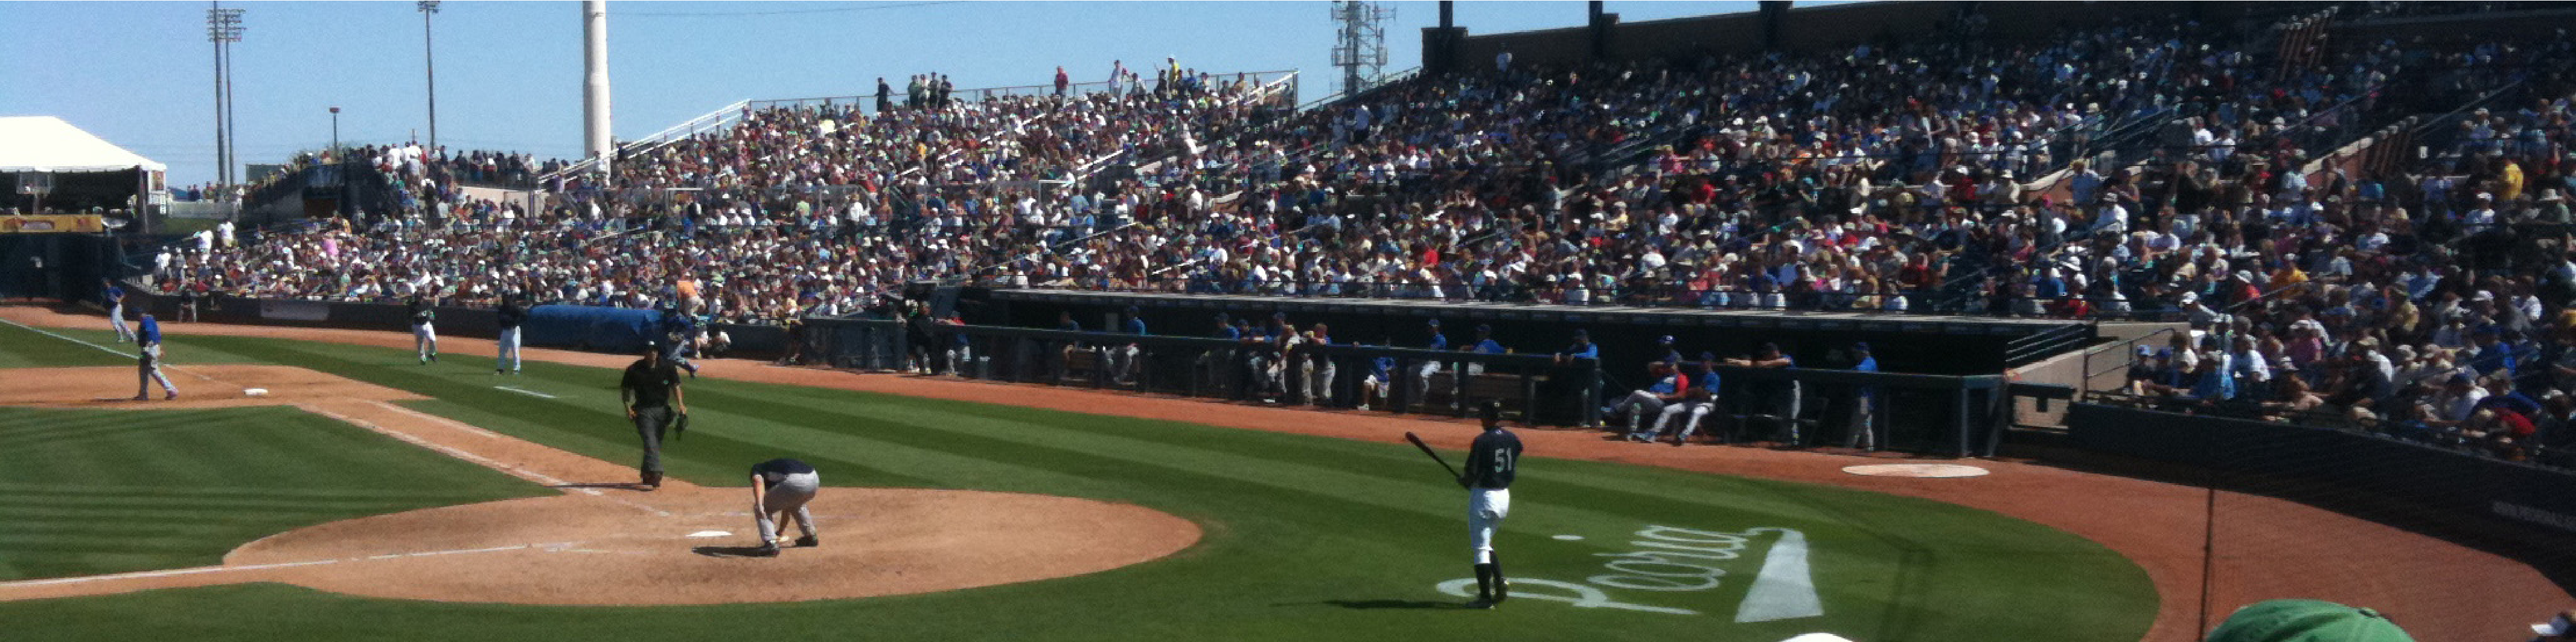
\includegraphics[width=\textwidth]{sampleteaser}
%  \caption{Seattle Mariners at Spring Training, 2010.}
%  \Description{Enjoying the baseball game from the third-base
%  seats. Ichiro Suzuki preparing to bat.}
%  \label{fig:teaser}
%\end{teaserfigure}

\maketitle
%
%
%

\section{Introduction}
\label{sec:intro}

The Elliptic Curve Digital Signature Algorithm (ECDSA) \cite{Johnson2001, ansi2005} is a digital signature scheme based on the elliptic-curve cryptography (ECC),
    widely used in many popular applications, such as TLS \cite{rfc5246}, OpenPGP \cite{openpgp2007}, smart card \cite{smartcard2007}, and Bitcoin \cite{bitcoin2008}.
The core operation of ECDSA sign/verify is the scalar multiplication of a base point (or generator) over elliptic curves
    by a random nonce (or ephemeral key).
 And the security of ECDSA relies on the intractability of the elliptic curve discrete logarithm problem (ECDLP) that
 the inability to compute the scalar (ephemeral key) given the original (base) and product points.

However, in actual implementations, the ephemeral key and the scalar multiplication need careful protection.
Side channel attacks can obtain the information on the ephemeral key during the scalar multiplication.
Furthermore, as long as some bits of the ephemeral key are leaked,
    the ECDSA private key will be recovered \cite{Nguyen2001,HG2001,Nguyen2002,Nguyen2003}.

The partial ephemeral key exposure attack was first proposed by Howgrave-Graham and Smart~\cite{HG2001} in 2001 to recover the whole DSA private key.
It was improved by Nguyen and Shparlinski \cite{Nguyen2002} and extended to ECDSA \cite{Nguyen2003}.
The basic idea is to construct a Hidden Number Problem (HNP) with the partial knowledge of the ephemeral keys,
 and then reduce to the Closest Vector Problem (CVP) or the Shortest Vector Problem (SVP) in a lattice to calculate the private key.
In 2007, the Extended Hidden Number Problem (EHNP)~\cite{ehnp} was introduced as another way to construct the problem to be solved in the lattice to recover the private key using the partial ephemeral key information.

While the cache side channel attack is an efficient way to obtain the partial information of the ephemeral key.
With the Flush+Reload cache side channels \cite{flushreload},
 attackers can get a "double-add" chain and extract some useful information about the ephemeral key.
	Benger et al. \cite{Benger2014} extracted the LSBs of the ephemeral keys from the chain and constructed an HNP instance to recover the ECDSA private key from about 200 signatures.
In 2015, Van de Pol et al.~\cite{Van2015} improved Benger's attack,
 which exploited the positions of higher half non-zero digits of the wNAF representations of the ephemeral key extracted from the "double-add" chain.
In 2016,
Fan et al.~\cite{Fan2016} extracted and utilized the information from the the "double-add" chain to
construct the EHNP to recover the private key of ECDSA.
The number of signatures needed is reduced to $4$.
In 2017, Wang et al.~\cite{Wang2017} exploited the positions of two non-zero digits together with the length of the wNAF representation of the ephemeral key to construct an HNP instance. They need 85 signatures to recover the private key.
%��һ��������Ҫ�޸�

%ֻ�Ƕ����ݷ��������˸Ľ�����û�л�ø��������

The above works extracted the information in the wNAF representation of the ephemeral key.
They tried to make better use of the data achieved through the side channels and construct more effective lattice attacks
 to recover the private key.
They extracted the least non-zero digit \cite{Benger2014}, half non-zero digits \cite{Van2015}, all non-zero digits \cite{Fan2016} or two non-zero digits with the total length~\cite{Wang2017}.
In summary,
all information exploited in these attacks are the positions of the non-zero digits,
 and no more extra information about the ephemeral key is extracted from the side channels.
Although the lattice attacks are different in these works,
     no effort and improvement have been made to achieve and exploit more information.

In our paper, we focus on ECDSA with the wNAF representation of the ephemeral key.
%, especially the implementation in the OpenSSL library.
 We propose a new method to recover the ECDSA private key from the information leaked through side channels.
We try to not only make better use of the information achieved from side channels,
  but also to extract different information from the side channels.
First, we analyse the implementation code of ECDSA in OpenSSL
 and find that
the invert function is another exploitable vulnerability in the implementation of the scalar multiplication.
It inverts a number so that the subtraction is replaced by addition and the space storing the precomputed points is reduced by half.
In the calculation, if the sign of current non-zero digit of the ephemeral key is opposite to the previous one, the invert function is called, and the absolute value of this digit is used to index the precomputed points. Otherwise, the invert function is not called.
It helps us to determine the sign of the non-zero digits of the wNAF representation.
 % by exploiting the \emph{$EC\_POINT\_invert()$} function we can improve the cache side channel attacks.
So we obtain the sign of the non-zero digits in the wNAF representation of the ephemeral key by adding a monitor to the invert function.
 Thus, we achieve more information about the ephemeral key compared to previous attacks.
After that, we manage to recover the consecutive bits at the position of every non-zero digits of the ephemeral key based on the information obtained from the cache side channels.
Finally, we construct an EHNP \cite{} instance making use of all the consecutive bits of the ephemeral key.
We recover the ECDSA private key by converting it to the SVP problem and solving it with lattice reduction algorithms.

This attack is applied to the secp256k1 curve in OpenSSL 1.1.1b in this paper.
We choose the Flush+Flush~\cite{gruss2016flush} attack to monitor the functions of double, add and invert.
By monitoring the  invert function
	in addition to the double and add functions in OpenSSL, %	we obtain the ``double-add-invert'' chain.
we successfully extract whether each digit of the ephemeral key is zero or not,
 and determine the signs of the non-zero digits. % from this chain.
Then we use the BKZ \cite{Schnorr1994} algorithm to solve the EHNP instance,
    and effectively recover the ECDSA private key.
If the result of the Flush+Flush attack is perfect, we only need $2$ signatures to recover the private key with a probability of $3\%$.

Through the cache side channel, we get the information about the positions and the signs of all non-zero digits of the ephemeral key.
Compared to previous works, our method obtains more information about the ephemeral key, i.e. the signs of all non-zero digits.
We extract $153.2$ bits on average per signature for 256-bit ECDSA, which makes only $2$ signatures are enough to recover the ECDSA private key.
To make better use of the obtained information of the non-zero digits,
 we exploit them to extract sequences of consecutive bits of $k$ and construct the lattice attack.
We obtain multiple consecutive bits of the ephemeral key by converting the wNAF representation to the binary representation.
And then, we use these consecutive bits to construct the EHNP instance.
To the best of our knowledge, it is the first time to obtain and exploit all the
signs of the wNAF representation in the side channel attacks against ECDSA
and our attack needs the least number of signatures to recover the ECDSA private key.

Our contributions are summarized as follows:
\begin{itemize}
  \item
  We present a new lattice attack to recover the private key of ECDSA with the wNAF representation.
  First, we
    improve the cache side channel attacks by monitoring
      the invert function.
      It is the first work to exploit the sign of the non-zero digits of the ephemeral key in side channel attacks.
   Second, for the data from the cache side channel, we do not use them to construct the EHNP instance directly,
   as in previous works.
    We obtain multiple consecutive bits of the ephemeral key by converting the wNAF representation to the binary representation.
Finally, we use these consecutive bits to construct the EHNP instance.
The private key is recovered by solving the EHNP instance using lattice reduction algorithm.
  \item
    We apply our method to the secp256k1 curve in OpenSSL1.1.0.
     Through the cache side channel, $153.2$ bits of information per signature are obtained on average.
    The experiments show that only $2$ signatures are enough to recover the private key with a probability of $3\%$.
\end{itemize}

The rest of this paper is organized as follows.
Section \ref{sec:background} presents some preliminaries.
Section \ref{sec:attack} provides the details about our attack,
and Section \ref{sec:impl&exper} shows the implementation details and the experimental results.
Section \ref{sec:discussion} contains some extended discussions.
Section \ref{sec:relatedwork} introduces some related works.
Section \ref{sec:conclusion} draws the conclusion.

%ECDSA���㷺Ӧ��
%������Բ������ɢ��������
%�㷨���������Ա�����
%������ʵ����ȴ������׷���©��
%��˺ܶ���ͨ�����ŵ���������ȡ����ʵ���ϵ�й¶����Ϣ��������Կ�ָ���
%Cache���ŵ������ڽ������õ��㷺Ӧ��
%
%OpenSSL��ʵ����Ӧ����㷺��ʵ�֡�
%���У����������ϵ���Բ���ߣ�ʹ�õ���wNAF�㷨ʵ�ֵı����˷���
%XX�꣬����˶����ַ�ʽ�ĵĹ���
%XX������ʹ��Flush+Reload������ȡ�˶������ݣ������˸񹥻�
%������
%�����ǵ������У�����ʹ���ˡ��������ˡ�����
%�ﵽ�ˡ�����
%�ܵ���˵�����ĵĹ������£�
%1��
%2��
%
%���µ�ʣ�ಿ��������֯���ڶ��¡�������


\section{Preliminaries and Related Works}
\label{sec:background}
In this section, we first present the basic knowledge about the ECDSA and its implementation using the wNAF representation in OpenSSL.
Then, we describe the attack method of the cache side channels.
Also, the hidden number problem and the extended hidden number problem are introduced to utilize the data obtained from cache side channels.
Finally, we provide the related works.

\subsection{The Elliptic Curve Digital Signature Algorithm}
\label{intro_ecdsa}
ECDSA \cite{Johnson2001, ansi2005} is the migration of the Digital Signature Algorithm (DSA) \cite{DSS186} from the multiplicative group of a finite field to the group of points on an elliptic curve.

Let $E$ be an elliptic curve defined over a finite field $\mathbb{F}_{p}$ where $p$ is prime.
$G \in E$ is a fixed point of a large prime order $q$, that is $G$ is the generator of the group of points of order $q$.
These curve and point parameters are publicly known.
The private key of ECDSA is an integer $\alpha$ that satisfies $0 < \alpha < q$,
 and the public key is the point $Q = \alpha G$.
Given a hash function $h$, the ECDSA signature of a message $m$ is computed as follows:
\begin{enumerate}
  \item
    Select a random ephemeral key $0 < k < q$.
  \item
    Compute the point $(x, y) = kG$, and let $r = x$ mod $q$;
    if $r = 0$, then go back to the first step.
  \item
    Compute $s = k^{-1} (h(m) + r\cdot\alpha)$ mod $q$;
    if $s = 0$, then go back to the first step.
\end{enumerate}

The pair $(r, s)$ is the ECDSA signature of the message $m$.
For ECDSA signature, the ephemeral key $k$ must be kept random and secret.
The equation in the third step shows the private key can be computed if $k$ is leaked.
%If some signatures use the same $k$, or the random number generator in use is predictable, attackers can obtain the private key directly. ������飬�������޹أ���ͬk
Even if a portion of $k$ is known, the private key can be recovered by lattice attacks.
Therefore, the scalar multiplication $kG$ becomes the target of most attackers. % who expect to get the information about $k$.

%Given the knowledge of the ephemeral key k and all the
%known information of (s, r,m), the secret key can be easily
%recovered by
%�� = r?1(s �� k ? H(m)) mod q .


\subsection{The Scalar Multiplication using wNAF Representation}
\label{intro_wnaf}
%wnaf ��ʲô
%K �������� P �Ƕ������� K�ϵ���Բ���� E(K)�ϵĵ㣬k��һ��������,������Բ�����ϵ�ļӷ���ʽ����P��������� k��, k ��Ϊ������ kP��Ϊ��Բ���ߵ�ˣ�������˷�

Scalar multiplication $kG$ on the elliptic curve means that the point $G$ is added to itself $k$ times,
where $G$ is a point defined on the elliptic curve over the finite field,
 and the scalar $k$ is a big integer.
There are several algorithms to implement the scalar multiplication.
In OpenSSL, scalar multiplication in the prime field is implemented using the wNAF representation \cite{GORDON1998129,Miyaji1997,Koyama1002,Solinas2000} of the scalar $k$.
In wNAF, a number $k$ is represented by a sequence of digits which is either zero or an odd number satisfying $-2^{w} < k_{i} < 2^{w}$,
 where $w$ is the window size. In this representation, any  non-zero digit  is followed by at least $w$ zero digits.
The value of $k$ can be expressed as $k = \sum{2^{i} k_{i}}$.
Algorithm \ref{alg:wnaf} introduces the concrete method for converting a scalar into its wNAF representation.

\renewcommand{\algorithmicrequire}{\textbf{Input:}}
\renewcommand{\algorithmicensure}{\textbf{Output:}}

 \begin{algorithm}[t]
        \caption{Conversion to wNAF Representation}
        \label{alg:wnaf}
        \begin{algorithmic}[1]
            \Require Scalar $k$, window size $w$
            \Ensure $k$ in wNAF: $k_0$, $k_1$, $k_2$, ...

            \State $i \gets 0$
            \While{$k > 0$}
                \If {$k$ mod $2 = 1$}
                    \State $k_i \gets k$ mod $2^{w+1}$
                    \If {$k_{i} \geq 2^{w} $}
                        \State $k_{i} \gets k_{i} - 2^{w+1}$
                    \EndIf
                    \State $k \gets k - k_{i}$
                \Else
                    \State $k_{i} \gets 0 $
                \EndIf
                \State $k \gets k/2 $
                \State $i \gets i+1 $
            \EndWhile
        \end{algorithmic}
    \end{algorithm}

%������ת����naf
%ת������μ�������˷�
For the scalar multiplication using wNAF representation, during the initialization phase,
  a window size $w$ is chosen, and the points $\{\pm G, \pm 3G, ..., \pm(2^{w}-1)G\}$ are precomputed and stored. 
Then, for each $k$, after converting it to the wNAF form, the multiplication $kG$ is executed as described in Algorithm \ref{alg:kg}.

\renewcommand{\algorithmicrequire}{\textbf{Input:}}
\renewcommand{\algorithmicensure}{\textbf{Output:}}

 \begin{algorithm}[t]
        \caption{Implementation of $kG$ Using wNAF}
        \label{alg:kg}
        \begin{algorithmic}[1]
            \Require Scalar $k$ in wNAF: $k_0$, $k_1$, ..., $k_{l-1}$ and precomputed points $\{\pm G, \pm 3G, ..., \pm(2^{w} - 1)G\}$
            \Ensure $kG$

            \State $Q \gets G$
            \For{$i$ from $l-1$ to $0$}
                \State $Q \gets 2\cdot Q$
                \If {$k_i \neq 0$}
                    \State $Q \gets Q + k_{i}G$
                \EndIf
            \EndFor
        \end{algorithmic}
    \end{algorithm}


From the Algorithm~\ref{alg:kg}, we can find that the if-then block (Line 4) is vulnerable to side channel attacks.
An attacker can use a spy process to monitor the conditional branches through side channels.
Then he can get a Double-Add chain, and determine  whether $k_i$ is zero or not based on this chain. 
The attacker can  use this  information to recover the  private key.

In OpenSSL, the bit length of $k$ is set to a fixed value$\lfloor\log_{2}{q}\rfloor + 1$ of by adding itself with $q$
or $2q$, which can resist the remote timing side channel attack \cite{Brumley2011}.
In most cases, the multiplication is done as $(k + q)G$, but it is still vulnerable in lattice attacks \cite{Dahmun2016}.

Also, OpenSSL uses the modified wNAF representation instead of the generalized one stated in Algorithm~\ref{alg:wnaf} to avoid length expansion in some cases and to make more efficient exponentiation.
The representation of modified wNAF is very similar to the wNAF.
Each non-zero coefficient is followed by at least $w$ zero coefficients,
 except for the most significant digit which is allowed to violate this condition in some cases.
As the modification on wNAF has little affects on the attack results,
%the use of modified wNAF affects the attack results little,
 we only consider the case of the generalized wNAF for clarity. %���һ����Ҫ�޸ģ�����һ����Ҫ�Ͷ�ƪ���¶Ա�����, ������Ҫ�ں��ʵ�λ�ü�������ʹ��256�����ߣ�window ��СΪ3


%�������һЩ�������������ж� ����ͨ�����ŵ���ȡ��Ϣ��
%
%ʵ���е�ʹ��k+q
\subsection{The Scalar Multiplication in OpenSSL}
\label{intro_smulinssl}
In OpenSSL versions between 0.9.7 and 1.1.0h~\cite{openssl}, the scalar multiplication with wNAF representation is implemented in the function \verb+ec_wNAF_mul()+.
The core computation of the function is shown in Algorithm  \ref{alg:smopenssl}.

\renewcommand{\algorithmicrequire}{\textbf{Input:}}
\renewcommand{\algorithmicensure}{\textbf{Output:}}

\begin{algorithm}[t]
        \caption{The Implementation of The Scalar Multiplication in OpenSSL}
        \label{alg:smopenssl}
        \begin{algorithmic}[1]
            \Require Scalar $k$ in wNAF $\{k_0$, $k_1$, ..., $k_{l-1}\}$ and precomputed points $\{G, 3G, ..., (2^{w} - 1)G\}$
            \Ensure $kG$
			
			\State $r \gets 0$, $is\_neg \gets 0$, $r\_is\_inverted \gets 0$
            \For{$i$ from $l-1$ to $0$}
            	\If {$r \neq 0$}
            		\State \Call{$EC\_POINT\_dbl$}{$r$}     {    }  $//$ $double$
                \EndIf
                \If {$k_i \neq 0$}
                	\State $is\_neg \gets (k_i < 0)$
                	\If {$is\_neg$}
                		\State $k_i \gets -k_i$
                	\EndIf
                	\If {$is\_neg \neq r\_is\_inverted$}
                		\If {$r \neq 0$}
                			\State \Call{$EC\_POINT\_invert$}{$r$}   {    }  $//$ $invert$
                		\EndIf                	
                    	\State $r\_is\_inverted \gets !r\_is\_inverted$
                	\EndIf
                	\If {$r = 0$}
                		\State $r \gets $ \Call{$EC\_POINT\_copy$}{$k_{i}G$}
                	\Else
                		\State $r \gets $ \Call{$EC\_POINT\_add$}{$r, k_{i}G$} {   }  $//$   $add$
                	\EndIf
                \EndIf
            \EndFor
            \State \Return r
        \end{algorithmic}
\end{algorithm}

In this function, it iterates the $k$ from the most significant digit to the least significant digit in its wNAF representation.
 In each digit, it performs a double operation (the \verb+EC_POINT_dbl()+ function).
  If the digit is not zero, it runs into the if-then block in Line 6, and first determines whether an invert function is needed. % to execute.
   The invert function is to compute the inverse of a point (the internal value of $kG$ here).
If the sign of the non-zero digit $k_i$ is opposite to the previous  non-zero digit,
 the invert operation (\verb+EC_POINT_invert()+) is performed (Line 13),
which makes it only need to precompute and store the points $\{G, 3G, ..., (2^{w} - 1)G\}$, and saves a half of storage space.
Then, an addition operation (the \verb+EC_POINT_add()+ function) is invoked to add the internal value of $kG$  with  a precomputed point indexed by  the
absolute value of the digit.


From Algorithm \ref{alg:smopenssl}, it can be found that two conditional branches are vulnerable.
In each loop, the double operation is always performed.
But the add operation is only performed when the digit is not zero and the invert operation is only performed when the sign of the digit is opposite to previous one.
Therefore, if a spy process can obtain the execution sequence of
  the double and addition operations,
one can determine whether each digit of $k$ is zero or not according to this sequence.
Also,  the execution sequence of the invert operation can be used to determine the signs of the non-zero digits combining with the former sequence.



\subsection{Cache Side Channel Attacks}
\label{intro_cacheattack}
Cache side-channel attacks, firstly proposed in 2002~\cite{Page2002},  take advantage of the characteristic of cache activity
 that accessing data from caches is much faster than from memory.
Attackers exploit these time variations to deduce the operations of the target process and then infer the key information.

For the symmetric cryptography,
Tsunoo et al. \cite{Tsunoo2003Cryptanalysis} and Bernstein \cite{Bernstein2005Cache} proposed the first practical cache attacks on DES and AES, respectively.
 These methods statically analyze the relation between the overall execution time and lookup table indexes which are affected by the cache behavior.
Bonneau and Mironov \cite{Bonneau2006} showed how to exploit cache collisions to recover the  AES secret key.
In 2006, Osvik et al. \cite{Osvik2006} presented two access-driven attacks: Evict+Prime and Prime+Probe,
%Although the latter one proved to be significantly more efficient, both of them
to recover the AES encryption key used by an OpenSSL server.
 Ac{\i}i{\c{c}}mez et al.~\cite{ac2006} presented a trace-driven attack targeting AES that exploited the cache collision during the first round.
In 2011, Gullasch et al.~\cite{cachegame2011} first presented the access-driven attack on AES encryption by blocking the AES execution after each memory access using the process scheduling algorithm.
In 2014, Irazoqui \cite{Irazoqui2014} exploited the Flush+Reload technique to attack the AES.

For the asymmetric cryptography,
The works~\cite{Percival2005CACHEMF,Onur2007Yet} attacked RSA, by exploiting the data cache and the instruction cache respectively. % to obtain the leaked information.
Then
Brumley and Hakala \cite{Brumley2009} mounted an L1 data cache-timing attack to recover the 160-bit ECDSA private key by obtaining the LSBs of ECDSA ephemeral keys from the \verb+dgst+ tool in OpenSSL 0.9.8k.
 While Ac{\i}i{\c{c}}mez et al. \cite{Brumley2010} used an L1 instruction cache-timing attack to recover a 160-bit DSA private key in OpenSSL 0.9.8l from the same tool.
 In 2014 Yarom et al. proposed the Flush+Reload method using the L3 cache to attack RSA \cite{flushreload} and ECDSA~\cite{yarom2014recovering} private key.
Also, this method is improved to attack the ECDSA with wNAF representation in \cite{Benger2014,Van2015,Fan2016}.
%Benger et al.~\cite{Benger2014} and Van de Pol et al. \cite{Van2015} demonstrated the viability of the Flush+Reload technique to recover ECDSA encryption keys.
%Fan et al. \cite{Fan2016} proposed a new way of extracting and utilizing information from the Flush+Reload attack.
In 2006, the variants of Flush+Reload are presented such as Flush+Flush \cite{gruss2016flush} and Prime+Abort \cite{disselkoen2017prime+abort}.
They exploited different methods to observe the cache access patterns to recover the private key.
 %and could be used in both local and virtualized environments.

In cloud computing environment, various cache side channel attacks are also proposed.
In 2009, Ristenpart et al.~\cite{get-off-my-cloud} presented methods to co-locate two virtual machines (VMs) and successfully recovered keystrokes from the co-resident victim's VM by the cache side-channel attacks.
Based on this work~\cite{get-off-my-cloud}, various attacks are extended to the co-resident VMs.
%This work was the basis of the cache attacks cross VMs because the caches were only shared with co-resident VMs.
For instance, Flush+Reload was used to attack AES \cite{Irazoqui2014} and RSA\cite{flushreload} in the cross-VM scenario.
Also, the Prime+Probe method was
adapted to work in virtualized environments by Zhang et al.~\cite{YinqianZhang2012-cross-vm} and Liu~\cite{liu2015last} to recover ElGamal encryption keys.
Irazoqui et al.~\cite{fine2014} recovered AES keys in virtualized environments with Bernstein's attack.

%Many attack methods are proposed \cite{Bonneau2006, Bernstein2005Cache, Osvik2006, cachegame2011, flushreload}
% since it is demonstrated feasible in theory \cite{Page2002}.
Here, we provide the detailed processes of Flush+Reload \cite{flushreload} and Flush+Flush \cite{gruss2016flush},
 which can be used to monitor the execution sequence of functions in the implementation of ECDSA.
%�ڽ�Щ����о��У����������Ĺ����ܵ��о����ǵ���������Ϊ����и��ߵĹ������ȣ��ܹ���׼ȷ�Ļ�ȡ��Ŀ����̶�cache�ķ���������Լ������ʹ�ó�������������⻯�ƻ������й����������������Ƕ����ֵ��͵ķ��������������н��ܣ������ֹ����ͱ�����ء�

The Flush+Reload attack \cite{flushreload} employs a spy process to monitor whether the specific memory lines have been accessed or not by the victim process.
So this attack relies on shared memory between the spy and the victim processes.
For attacks in the same machine, the spy can map the victim program file, the victim data file or shared libraries into its own address space to share these pages with the victim.
While in the virtualization environments, the page de-duplication technique of the VMM ensures the page sharing between the spy and the victim.
%���LLC����Ҫдһ��
The execution of such an attack consists of three phases:
\begin{itemize}
  \item
    \textbf{Flush:}
    The attacker uses the \verb+clflush+ instruction to flush the desired memory lines out from the caches.
    This ensures that these lines are accessed from the memory instead of the caches for the next time.
  \item
    \textbf{Wait:}
    the attacker waits a moment while the victim is running.
  \item
    \textbf{Reload:}
    This phase detects whether the victim accesses the memory lines flushed in the first phase during the waiting time.
    The attacker accesses the desired memory lines to reload them into caches, and measures the time.
%From the reload time, the attacker determines whether the memory lines are accessed by the victim.
    The longer reload time means that the victim does not access the data and the attacker has to reload the data from the memory.
    Otherwise, it means that the victim accesses the data.
%    So these memory lines are accessed by the victim during the waiting time.%��Ҫ����
\end{itemize}

The Flush+Flush attack \cite{gruss2016flush} also assumes the shared memory.
%Unlike measuring the reload time directly affected by the cache access,
It relies on the execution time of the \verb+clflush+ instruction,
  which is affected by whether the to-be-flushed data are cached or not.
The execution time of \verb+clflush+ is shorter if the data are not cached
 and longer if the data are cached.
So according to this time, the attackers determine the victim's cache activities.

In general, the Flush+Flush attack also consists of three phases.
The first two phases are the same as in the Flush+Reload attack.
But in the third phase, it flushes the cache again and measures the flush time instead of the reload time.
%As the third phase flushes the caches, it doubles as the first phase for subsequent observations.

%��һ��F+F �� F+R���жԱȣ����Ӹ�Ч�����ȸ��ߣ�F�׶ο��Ե�������һѭ����F��
The execution time of \verb+clflush+ is less than the reload time on average,
    and the first and the third phase are merged together in the Flush+Flush attack.
  Therefore, the Flush+Flush attack is more accurate than the Flush+Reload attack.
%Thus, the Flush+Flush attack has a better accuracy.
%Furthermore, compared with the Flush+Reload attack,
%the Flush+Flush attack does not trigger prefetches when monitoring consecutive memory lines, otherwise, it may affect the validity of the attack.


%��һ��Ҫ�Ͷ�ƪ���½��жԱȸĽ���f+r������Ҫ����
%f+r���㷨α���뿼���費��Ҫ���ӡ�

\subsection{The Hidden Number Problem and Lattice Attack}
\label{intro_hnp}

For the wNAF algorithm,
 the if-then block (Line 4 in Algorithm~\ref{alg:kg}) is vulnerable to side channel attacks.
An attacker can use a spy process to monitor the conditional branches through side channels.
Then he can get a Double-Add chain, and determine whether  $k_i$ is zero or not from this chain.
But this is not enough to determine the complete ephemeral key,
 only some bits of the ephemeral key are obtained.
The attacker then use this extracted information to launch a lattice attack to recover the private key.


The Hidden Number Problem (HNP) is first presented by Boneh and Venkatesan~\cite{boneh1996} in 1996.
It is used to recover the secret key of Diffie-Hellman key exchange~\cite{boneh1996}, DSA~\cite{HG2001} and ECDSA~\cite{Nguyen2003}, given some leaked consecutive bits of the ephemeral key.
Given a prime number $q$ and a positive $l$,
 and let $t_1, t_2, ..., t_d$ be randomly chosen, which are uniformly and independently in $\mathbb{F}_q$.
The HNP can be stated as follows:
  recovering an unknown number $\alpha \in \mathbb{F}_q$ such that the known number pairs $(t_i, u_i)$ satisfy
  $$v_i = |\alpha t_i - u_i|_{q} \leq q/2^{l+1}, \ \ \ \ 1 \leq i \leq d,$$
   where $|\cdot|_q$ denotes the reduction modulo $q$ into range $[-q/2, ..., q/2)$.
If $|\alpha t - u|_{q} \leq q/2^{l+1}$ is satisfied,
the integer $u$ represents the $l$ most significant bits of $\alpha t$ which is defined as ${MSB}_l(\alpha t)$.


The Extended Hidden Number Problem (EHNP) introduced in~\cite{ehnp} is stated as follows, which also can be used to recover the ECDSA private key~\cite{Fan2016}.
Let $N$ be a prime number. Given $u$ congruences
$$
\beta_{i}x + \sum_{j=1}^{l_i}{a_{i,j}k_{i,j}} \equiv c_i \ \ \ \bmod N, \ \ \ 1 \leq i \leq u \ ,
$$
where $k_{i,j}$ and $x$ are unknown variables satisfying $0 \leq k_{i,j} \leq 2^{\varepsilon_{i,j}}$ and $0 < x < N, \beta_i, a_{i,j} , c_i, l_i \text{ and } \varepsilon_{i,j} $ are all known.
%The EHNP can be further converted to the approximate SVP in some suitable lattice to find the unknown $x$ (the hidden number) which satisfies the conditions above.
The EHNP is to find the unknown $x$ satisfying the conditions above.

For ECDSA algorithm, attackers take advantage of the equation $s = k^{-1} (h(m) + r\cdot\alpha) \bmod q$.
Based on the partial information about the ephemeral key obtained by the attackers through the cache side channels,
 they transform this equation to satisfy the form of HNP or EHNP.
   Then the private key as the hidden number can be recovered
      by solving the SVP/CVP problem in lattice converted from HNP or EHNP using the lattice reduction algorithm such as LLL \cite{Lenstra1982} or BKZ \cite{Schnorr1994}.

%we can use  algorithm to solve the SVP problem, while use Babai \cite{Babai1986} algorithm or Enumeration technique to solve the CVP problem.

%��һ��˵����cache�������Ի����Ϣ��Ȼ����ת����hnp��������⡣
%For the ECDSA algorithm implemented by OpenSSL with the wNAF,
%  the attackers can obtain some consecutive bit fragments of the ephemeral key $k$ through the cache side channels.
%Then, the problem of recovering the secret key can be transformed to the HNP problem.
% The attackers can recover the secret key by solving the HNP problem using lattice reduction algorithms.

%
%The HNP problem can be converted to the CVP/SVP problem in lattices
% and solved by the lattice reduction.
%Here we provide a brief introduction.
%For more details on lattice, please refer to the literature \cite{latticereduction2000}.
%Consider the Euclidean space $\mathbb{R}^{d}$
% and let $B = \{\mathbf{b_1}, \mathbf{b_2}, ..., \mathbf{b_z}\}$ be a set of linearly independent vectors in $\mathbb{R}^d$.
%The set of vectors
%$$
%L = L(B) = \{\sum_{i=1}^{z}{\beta_i\mathbf{b_i}} \  |\ \beta_i \in \mathbb{Z} \}
%$$
%is the lattice generated by $B$.
%The set $B$ is called a basis of $L$, and $L$ is spanned by $B$.
%The number $z$ representing the number of vectors in $B$ is the dimension or rank of $L(B)$.
%If $z = d$, the lattice $L(B)$ is a full-dimension lattice.
%As the lattice is a set of vectors,
%  the norm of the shortest non-zero vector is called the first minima and denoted by $\mathbf{\lambda_1}(L)$.
%That is, $\mathbf{\lambda_1}(L) = \min\{\|\mathbf{u}\| \ |\  0 \neq \mathbf{u} \in L\}$, where $\|\mathbf{u}\|$ denotes the Euclidean norm of the vector $\mathbf{u}$.
%The problem of finding a non-zero vector $\mathbf{v} \in L$ with the minimal norm is called the shortest vector problem (SVP).
% While for a lattice $L$ and an arbitrary vector $\mathbf{v} \in \mathbb{R}^d$,
% the problem of finding a lattice vector $\mathbf{u} \in L$ of minimal distance from $\mathbf{v}$ is called the closest vector problem (CVP) similarly.
%  In other words, finding a vector $\mathbf{u}$ satisfied $\|\mathbf{u}\| = \min\{\|\mathbf{u} - \mathbf{v}\| \ |\   \mathbf{u} \in L\}$.
%
%Exploiting lattices to solve the HNP problem, we construct a $d+1$ dimensional lattice $L(B)$ spanned by the rows of the following matrix:
%$$B =
%\left(
%  \begin{array}{ccccc}
%    q & 0 & \cdots & 0 & 0 \\
%    0 & q & \ddots & \vdots & \vdots \\
%    \vdots & \ddots & \ddots & 0 & \vdots \\
%    0 & \cdots & 0 & q & 0 \\
%    t_1 & \cdots & \cdots & t_d & 1/2^{l+1} \\
%  \end{array}
%\right).
%$$
%Considering the vector $\mathbf{h} = (\alpha t_1 \bmod q, ..., \alpha t_d \bmod q, \alpha /2^{l+1})$,
% it can be obtained by multiplying the last row vector of $B$ by $\alpha$ and then subtracting appropriate multiples of the first $d$ row vectors.
%Thus the vector $\mathbf{h}$ belongs to $L(B)$.
%We call $\mathbf{h}$ the hidden vector because the last coordinate of $\mathbf{h}$ discloses the hidden number $\alpha$.
%Let the vector $\mathbf{u} = (u_1, ..., u_d, 0)$,
% so the distance between $\mathbf{h}$ and $\mathbf{u}$ is $\|\mathbf{h} - \mathbf{u}\| \leq q\sqrt{d+1}/2^{l+1}$.
%Because the lattice determinant of $L(B)$ is $q^d/2^{l+1}$,
%  the vector $\mathbf{h}$ is very close to the vector $\mathbf{u}$.
%Solving the CVP problem with input $B$ and $\mathbf{u}$ reveals the vector $\mathbf{h}$,
% hence the private key $\alpha$ is recovered.
%
%Because solving the CVP instance requires exponential time in the lattice rank,
% we can use the embedding technique \cite{Nguyen1999} to transform it to an SVP instance which just requires the polynomial time to solve.
%We construct a $d+2$ dimensional lattice $L(B')$ spanned by the rows of the matrix
%$$B' =
%\left(
%  \begin{array}{cc}
%    B & 0 \\
%    \mathbf{u} & q/2^{l+1} \\
%  \end{array}
%\right).
%$$
%Similarly, the vector $\mathbf{h}' = (\alpha t_1 - u_1 \bmod q, ..., \alpha t_d - u_d \bmod q, \alpha /2^{l+1}, -q/2^{l+1})$ belongs to the lattice $L(B')$.
% Its norm satisfies that $\|\mathbf{h}'\| \leq q\sqrt{d+2}/2^{l+1}$,
%  while the lattice determinant of $L(B')$ is $q^{d+1}/2^{2l+2}$.
%   This indicates that the vector $\mathbf{h}'$ is a very short vector.
%Note that this lattice also contains another vector $(-t_1, ..., -t_d, q, 0)\cdot B = (0, ..., 0, q/2^{l+1}, 0)$,
% which is most likely the shortest vector of the lattice.
%So we expect the second vector in a reduced basis of the lattice is equal to $\mathbf{h}'$ with a ``good'' chance for a suitably strong lattice reduction algorithm.
%Then we can acquire the hidden number $\alpha$ by solving the SVP problem.


\subsection{Partial Nonce Disclosure Attacks on DSA/ECDSA}
Various works are proposed to exploit partial nonce disclosure to recover long-term private keys
 of the algorithms based on the discrete logarithm problem. 
In this section, we provide a brief description of these works.
%They can be classified into (1) ones proving that exploiting the partial information can recover the whole private key,
% and (2) ones that focus on how to obtain the partial information and construct appropriate lattice attacks to recover the private key.
%Some of them focus on
%proving that exploiting the partial information can recover the whole private key.
% And others pay more attention on how to obtain the partial information and construct appropriate lattice attacks to recover the private key.

% first
Boneh and Venkatesan \cite{boneh1996} initially investigated to use the partial information of the ephemeral key to construct an HNP problem and recovered the private key of Diffie-Hellman by solving it using the lattice reduction algorithm.
 Howgrave-Graham and Smart \cite{HG2001} extended this work to recover the DSA private key by  constructing an HNP instance from leaked LSBs and MSBs of the ephemeral key.
  Nguyen and Shparlinski \cite{Nguyen2002} proved that
      knowing the $l \geq 3$ LSBs, the $l+1$ MSBs  or any $2l$ consecutive bits of a certain number of ephemeral keys was enough for recovering the DSA private key.
 They recovered  a $160$-bit DSA key only using the $3$ LSBs of a certain number of ephemeral keys.
 Further, they extended these results to ECDSA~\cite{Nguyen2003}.
Liu and Nguyen \cite{Liu2013} improved the results that only 2 LSBs were required for breaking a 160-bit DSA key.

%In 2014, Benger et al. \cite{Benger2014} extended the technique in \cite{Nguyen2002} to use a different length of leaked LSBs for each signature.
% They recovered the secret key of OpenSSL's ECDSA implementation for the curve secp256k1 using about $200$ signatures.
%Van de Pol et al. \cite{Van2015} exploited the property of the modulus in some elliptic curves so that they could use all of the information leaked in the top half of the ephemeral keys to construct the HNP instance, allowing them to recover the secret key after observing only $14$ signatures.
%Fan et al. \cite{Fan2016} transformed the problem of recovering the secret key to the extended hidden number problem (EHNP)
%  which was solved by the lattice reduction algorithm.
%   Then the number of signatures needed was reduced to $4$.

%second
Brumley and Hakala \cite{Brumley2009} used an L1 data cache-timing attack to recover the LSBs of ECDSA ephemeral keys in OpenSSL 0.9.8k.
 They recovered a 160-bit ECDSA private key using the attack in \cite{HG2001} with  $2,600$ signatures ($8K$ with noise).
Analogously, Ac{\i}i{\c{c}}mez et al. \cite{Brumley2010} used an L1 instruction cache-timing attack to recover the LSBs of DSA ephemeral keys in OpenSSL 0.9.8l.
 It required $2,400$ signatures ($17K$ with noise) to recover a 160-bit DSA private key.
 Besides, both attacks required HyperThreading architectures.
In 2011, Brumley and Tuveri \cite{Brumley2011} mounted a remote timing attack on the implementation of ECDSA with binary curves in OpenSSL 0.9.8o.
 They obtained the MSBs of the ephemeral keys through the timing attack and recovered the private key after collecting information over 8,000 TLS handshakes.
In 2013, Mulder et al. \cite{Mulder2013} took advantage of a template attack to recover some LSBs of the ephemeral key.
They improved the Bleichenbacher's FFT-based (Fast Fourier Transform) attack by using BKZ for range reduction to solve the HNP problem.
Their attack could extract the entire private key using a 5-bit leak of the ephemeral key from 4 000 signatures.
%Benger et al. \cite{Benger2014} and Van de Pol et al. \cite{Van2015} used the Flush+Reload technique to acquire the information of the ephemeral key.
In 2014, Benger et al. \cite{Benger2014} extended the technique in \cite{Nguyen2002} to use a different length of leaked LSBs for each signature.
 They recovered the secret key of OpenSSL's ECDSA implementation for the curve secp256k1 using about $200$ signatures.
Then in 2015,
Van de Pol et al. \cite{Van2015} exploited the property of the modulus in some elliptic curves so that they could use all of the information leaked in the top half of the ephemeral keys to construct the HNP instance, allowing them to recover the secret key after observing only $14$ signatures.
In 2016, Allan et al. \cite{Allan2016} improved the results in \cite{Van2015} by using a performance-degradation attack to amplify the side-channel. The amplification allowed them to recover a 256-bit private key in OpenSSL 1.0.2a after observing only 6 signatures.
Fan et al. \cite{Fan2016} transformed the problem of recovering the secret key to the extended hidden number problem (EHNP)
 which was solved by the lattice reduction algorithm.
  Then the number of signatures needed was reduced to $4$.
Genkin et al. \cite{Genkin2016} performed electromagnetic and power analysis attacks on mobile phones.
 They showed how to construct HNP triples when the signature uses the low $s$-value.
Pereida et al. \cite{Pereida2016} showed that the DSA implementation in OpenSSL is vulnerable to cache-timing attacks due to a programming error,
 and exploited the vulnerability to attack against SSH (via OpenSSH) and TLS (via stunnel).
In 2017, Wang et al. \cite{Wang2017} exploited the HNP to recover the private key for the 256-bit curve using $85$ signatures using a few information from the Flush+Reload attack.
 Zhang et al. \cite{Zhang2017} extended  the attack in ~\cite{Nguyen2003} to SM2 Digital Signature Algorithm (SM2-DSA), which is a Chinese version of ECDSA.




%1 ʲô�Ǹ�

%2 ʲô�Ǹ���������

%3 HNP��������ø������



\section{Attacking ECDSA}
\label{sec:attack}
In this section, we propose a new method to recover the private key of ECDSA.
First, we analyse the invert function in the scalar multiplication with wNAF representation in the ECDSA algorithm.
 Then we use the invert function for improving the cache side channel attacks, from which the sign of the non-zero digits of $k$ is determined.
After that, we make use of the obtained information to recover the consecutive bits at the position of every non-zero digits of $k$.
Finally, we construct an HNP instance by the consecutive bits and transform it to the problem of solving the SVP/CVP in some lattice with the lattice reduction algorithms.

\subsection{Attacking wNAF through the Cache Side Channels}
\label{data_get}
First recalling the implementation of scalar multiplication in OpenSSL, it uses the invert function to
  compute the inverse element of a number.
Applying this function, the space of precomputed points is saved by half, only need to store $\{G, 3G, ..., (2^{w} - 1)G\}$.
As shown in Algorithm~\ref{alg:smopenssl},
it iterates $k$ from the most significant digit to the least significant digit.
In each digit, it performs a double function.
While if the digit is not zero, it first determines whether the invert function is executed.
 If the sign of the digit is opposite to the prior one, the invert function is called.
Then it indexes from the precomputed points using the absolute value of the digit and performs an addition operation.

Originally, the vulnerability comes from the double and add function.
The double function is called at every digit, and this reveals the digit sequence.
The add function is called just when the digit is not zero,
  which makes it possible to distinguish whether the digit is zero or not.
  That reveals the position of all the non-zero digits.
However,
 the invert function is also vulnerable, because it is called conditionally, either.
Only in the condition that the sign of the non-zero digit is opposite to the previous, the invert function will be performed.
Because we know the first non-zero digit is positive,
   the sign of all the non-zero digit can be deduced based on the execution of the invert function.


We use a spy process to monitor one memory line of the code of the double, add and invert functions while computing the scalar multiplication.
The time is divided into slots, and in each slot,
  the spy determines whether the three functions are performed or not by monitoring the cache hits/misses.
 Then we can obtain a ``double-add-invert" chain.
According to the ``double" and ``add" in this chain, we can determine whether each digit of $k$ is zero or not.
  That is what the original Flush+Reload attack does.
Also, based on the ``invert" in this chain, we can infer the sign of each non-zero digit.


Specific to the OpenSSL implementation (especially the OpenSSL1.1.1b used here),
  the double, add and invert function are implemented using  \verb+EC_POINT_dbl()+, \verb+EC_POINT_add()+ and \verb+EC_POINT_invert()+.
 The original cache side channel attack monitors the \verb+EC_POINT_dbl()+ and \verb+EC_POINT_add()+ function.
So as in our attack, we improve the original cache side channel attack by adding a new monitor to the \verb+EC_POINT_invert()+ function.
We use a spy process to monitor one memory line of the code of the three functions.
 In each time slot
  the spy determines whether the three functions are performed or not.
Then we get a new ``double-add-invert" chain through the cache side channel attack.

%���Ȼع˱����˷���ʵ�֣�ԭʼʵ�֡�
%Ȼ��invert���������������ʹ�õģ�����ʲô���á�
%©���������ô��ȥ���á�
%OpenSSL�����ǵ�ʵ�֣�
%�����ڹ�������ô����
%Ȼ��õ���ʲô


When we use the ``double-add-invert" chain to extract the digits of $k$,
the ``double" represents the double function is called,
and the ``add" represents the double and add functions are called both.
The ``invert" represents the invert function is called.
Therefore,
 the ``double" appears meaning that $k_i$ is zero
and the ``add" appears meaning that $k_i$ is not zero.
 Then we use the ``invert" to determine the sign of the $k_i$.
The sign of the $k_i$ is related to the previous non-zero digit.
First, the ``invert" comes out together with ``add".
 Then, if the ``invert" appears, it represents that the sign of this digit $k_i$ is opposite to the previous non-zero digit.
 While if the ``invert" does not appear when ``add" comes out, it represents that
the sign of this digit $k_i$ is the same as the previous non-zero digit.
 For the wNAF representation of $k$, the most significant digit is always positive.
 Thus we can determine the sign of all non-zero digits.
In this way, we obtain all the positions of the non-zero digits and the sign information of them.


% In our work, we implement the Flush+Flush attack to obtain the "double-add-invert" chain because it has a better precision.
%%���ﻹ��Ҫ�ٶ�˵���䣬ΪʲôҪ���ȸ��ߣ���Ϊreloadʱ�䳤������һ����������һ��slot�л���ʱ����࣬ �������ʧ�� flush��ʱ��̣�slot���Ը��̡�


%openssl��ʵ����XXXX��
%��ͳ�Ĺ�����double ��add���м��
%�������Ӷ�invert���м��
%Ȼ����εõ�digit��������Ϣ
%�����ǵ�ʵ���У�ͨ���Ա�f_f��f+r ѡ��f+f���й���


%�����ǣ������˷��������ʼλ�ú���Ҫ��

%���ţ�sign
%��һ���ò���һ��ͼ��˵��add-double��


\subsection{Consecutive Bits Recovery}
\label{data_proc1}
In this section, we introduce how to recover the consecutive bits at the position of every non-zero bits for the ephemeral key $k$, exploiting the information obtained from the side channel.

First, we denote the wNAF representation of $k$ as $k = \sum{k_{i}2^{i}}$,
 and the binary representation as $k = \sum{b_{i}2^{i}}$.
From the Algorithm \ref{alg:wnaf} we know that the position of $k_i$ in the wNAF representation is the same as $b_i$ in the binary representation.
 When we know the information about whether $k_i$ is zero and the sign of the non-zero $k_i$, we can simply determine some bits of $k$.
 For example, if we obtain the sign of the least non-zero $k_j$, we can infer that $b_j$ is one and $b_i$ is zero for $0\leq i<j$.
 But for arbitrary non-zero digits, it can not determine whether the bit is zero or one.

 Let $m$ and $m + n$ be the positions of two consecutive non-zero digits of the wNAF representation, and $w$ be the window size.
 That is, $k_m, k_{m+n} \neq 0$ and $k_{m+i} = 0$ for all $0 < i < n$.
 We analyse the transformation method between the binary and wNAF representation, getting the following result:

 \begin{align}
 &b_{m+n} = \left\{
 \begin{aligned}
 	&0,\,\;\ \   k_m < 0 \\
 	&1,\,\;\ \   k_m > 0
 \end{aligned}
 \right.  , \\
 &b_{m+i} = \left\{
 \begin{aligned}
 	&0,\,\;\ \   k_m > 0 \\
 	&1,\,\;\ \   k_m < 0
 \end{aligned}
 \right.
 ,\ \ \ \ \  w \leq i \leq n-1
 \end{align}
%����Ĺ�ʽ��©������Ҫ�������λ��m��Сʱ��bm

And if $m$ is the position of the least non-zero digit of $k$,
 \begin{align}
 &b_{i} = \left\{
 \begin{aligned}
 	&1,\,\;\ \   i = m \\
 	&0,\,\;\ \   0 \leq i < m
 \end{aligned}
 \right.  .
 \end{align}

In this way, at the position of every non-zero digit we can obtain $n - w + 1$ consecutive bits of $k$
 except at the  position of the least non-zero digit being $m+1$.
For the wNAF representation, every non-zero digit (except the least) is followed by at least $w$ zero values.
 The average number of non-zero digits of $k$ is $(\lfloor\log_{2}{q}\rfloor +1) /(w+2)$.
 The average distance between consecutive non-zero digits is $w+2$, i.e. on average $n = w + 2$.
 This means we can obtain $3$ consecutive bits on average at the every non-zero digit (except the least).
Based on \cite{Benger2014} on average we can get $2$ least significant bits of the ephemeral key.
Thus, on average we can obtain $3(\lfloor\log_{2}{q}\rfloor+1) /(w+2) - 1$ bits of the ephemeral key $k$ in total.
Meanwhile, because the minimal value of $n$ is $w + 1$, the minimal length of the consecutive bits is $2$.
This illustrates that all the sequences of consecutive bits obtained (except the least) are no less than $2$ bits.
For the \textbf{secp256k1} curve implemented in OpenSSL, $\lfloor\log_{2}{q}\rfloor  + 1= 256$, $w = 3$.
 Also, as introduced previous, the scalar multiplication uses $k+q$ instead of $k$ in most cases,
  so the total number of bits per signature we obtain is $3(\lfloor\log_{2}{q}\rfloor +2)/(w+2)-1 = 153.2$.
In theory, two signatures would be enough to recover the 256-bit private key as $2\times 153.2 = 306.4 > 256$.

%�����ټ�һС�Σ�������[����x]˵��ֻҪ֪��������2bit��Ϣ�����ܹ���������񹥻��ָ���Կ��
%��ˣ��Բ��ŵ��õ�������ʹ�����ǵķ����ָ���������������λ��ȫ�������Ա��õ������Ĺ�����

%���ȣ�k�Ķ����Ʊ�ʾ��k��wnaf��ʾ
%���ǵ�λ�Ƕ�Ӧ�ġ�
%������֪����digit��������Ϣ�󣬼򵥵ģ����ǾͿ����жϳ�ijЩ������λ�Ƕ�����
%Ȼ��������������ôȥȷ��
%�õ�һ����ʽ��
%
%Ȼ�����Ǿ͵õ���������bit��Ϣ
%ͨ��һ��ǩ���������ܹ���õ�bit��Ϊ��


\subsection{Constructing the Lattice Attack}
\label{data_proc2}
In this section, we transform the problem of recovering the private key to the HNP instance, and further convert to the CVP/SVP instance in a lattice.
Our method is based on the analysis from \cite{Nguyen2002}.
But we make some improvements on it.
First the length of the consecutive bits used to construct the lattice is variable while the prior work fixes the length, which may lose some information.
Second  in our method the position of consecutive bits is arbitrary in the ephemeral key and does not need to be fixed, while the prior work needs all the consecutive bits at the same position.
Finally from one signature we obtain multiple sequence of consecutive bits and all of them can be used for constructing the lattice as long as the length of the sequence is satisfied, while the prior work only generates one sequence of consecutive bits for one signature.

To construct a HNP instance using arbitrary consecutive bits, we need to use the following theorem\cite{Nguyen2002}:
\begin{theorem}
 \label{theorem1}
There exists a polynomial-time algorithm which, given $A$ and $B$ in $[1, q]$, finds $\lambda \in Z^{*}_{q}$ such that
$$
|\lambda |_q < B  \ \  \text{and} \ \  |\lambda A|_q \leq q/B .
$$
\end{theorem}
The value of $\lambda$ can be computed exploiting the continued fractions.

Recall the ECDSA signature, $s = k^{-1} (h(m) + r\cdot\alpha) \bmod q$.
We rewrite it as
\begin{equation}
\label{sig}
\alpha rs^{-1} = k - s^{-1}h(m)  \ \  \text{mod} \ \ q.
\end{equation}
Then assume that we have the $l$ consecutive bits of $k$ with the value of $a$, starting at some known position $j$.
 So $k$ is represented as $k = 2^{j}a + 2^{l+j}b +c$ for $0 \leq a \leq 2^l -1$, $0\leq b \leq q/2^{l+j}$ and $0 \leq c < 2^j$.
 We apply the theorem with $A = 2^{j+l}$ and $B = q2^{-j-l/2}$, to obtain $\lambda$ such that
$$
|\lambda |_q < q2^{-j-l/2}  \ \  \text{and} \ \  |\lambda 2^{j+l}|_q \leq q/2^{j+l/2} .
$$
Plugging the value of $k$ and multiplying by $\lambda$, Equation \ref{sig} is transformed to
$$
\alpha r\lambda s^{-1} = (2^{j}a - s^{-1}h(m))\lambda +(c\lambda + 2^{l+j}b\lambda)  \ \  \bmod \ \ q.
$$

 Let
 \begin{equation}
 \label{tu}
 \left\{
 \begin{aligned}
 	&t = \lfloor r\lambda s^{-1} \rfloor_q    \\
 	&u = \lfloor (2^{j}a - s^{-1}h(m))\lambda \rfloor_q
 \end{aligned}
 \right.
 \end{equation}
 where $\lfloor \cdot\rfloor_q$ denotes the reduction modulo $q$ into range $[0, ..., q)$.

We then have that
 \begin{equation}
\label{lattice}
    |\alpha t - u|_q < q/2^{(l/2-1)}
\end{equation}
This way, we transform to the a HNP instance.

In practice, OpenSSL uses $k+q$ as the ephemeral key. So the Equation \ref{tu} remains the same, but the Inequation \ref{lattice} turns into
 \begin{equation}
\label{lattice2}
    |\alpha t - u|_q < q/2^{(l/2-\log_{2}{3})}
\end{equation}

Note that, the Equation \ref{lattice2} represents that the $l/2-\log_{2}{3} -1$ most significant bits of $\lfloor\alpha t\rfloor_q$ is $u$, based on the definition of the HNP.
So it should satisfy that $l/2-\log_{2}{3} -1 \geq 1$, i.e. $l > 7$.
That means the length of the consecutive bits used to  construct the HNP instance should be larger than $7$,
although we could use all the partitions of the consecutive bits of the ephemeral key in theory.

Next we turn the HNP instance into the lattice problem.
We use $d$ triples $(t_i, u_i, l_i)$ to construct a $d+1$ dimensional lattice $L(B)$ spanned by the rows of the following matrix:
$$B =
\left(
  \begin{array}{ccccc}
    2^{l_1+1}q & 0 & \cdots & 0 & 0 \\
    0 & 2^{l_2+1}q & \ddots & \vdots & \vdots \\
    \vdots & \ddots & \ddots & 0 & \vdots \\
    0 & \cdots & 0 & 2^{l_d+1}q & 0 \\
    2^{l_1+1}t_1 & \cdots & \cdots & 2^{l_d+1}t_d & 1 \\
  \end{array}
\right).
$$
Considering the vector $\textbf{x} = (2^{l_1+1}\alpha t_1 \bmod q, ..., 2^{l_d+1}\alpha t_d \bmod q, \alpha)$,
 it can be obtained by multiplying the last row vector of $B$ by $\alpha$ and then subtracting appropriate multiples of the first $d$ row vectors.
Thus the vector $\textbf{x}$ belongs to $L(B)$.
Let the vector $\textbf{u} = (2^{l_1+1}u_1, ..., 2^{l_d+1}u_d, 0)$,
 so the distance between $\textbf{x}$ and $\textbf{u}$ is $\|\textbf{x} - \textbf{u}\| \leq q\sqrt{d+1}$.
While the lattice determinant of $L(B)$ is $2^{d + \sum{l_i}}q^d$,
 thus the vector $\textbf{x}$ is very close to the vector $\textbf{u}$.
By solving the CVP problem with the input $B$ and $\textbf{u}$, the vector $\textbf{x}$ is revealed,
 hence the private key $\alpha$ is recovered as it is the last element of the vector $\textbf{x}$.

To transform it to a SVP instance we use $d$ triples $(t_i, u_i, l_i)$ to construct a $d+2$ dimensional lattice $L(B')$ spanned by the rows of the matrix
$$B' =
\left(
  \begin{array}{cc}
     B\ \  &\  0\ \  \\
    \textbf{u}\ \ &\ q \ \  \\
  \end{array}
\right).
$$
Similarly, the vector $\textbf{x}' = (2^{l_1+1}(\alpha t_1 - u_1) \bmod q, ..., 2^{l_d+1}(\alpha t_d - u_d) \bmod q, \alpha, -q)$ belongs to the lattice $L(B')$.
 Its norm satisfies that $\|\textbf{x}'\| \leq q\sqrt{d+2}$,
  while the lattice determinant of $L(B')$ is $2^{d + \sum{l_i}}q^{d+1}$.
   This indicates that the vector $\textbf{x}'$ is a very short vector.
Note that this lattice also contains another vector $(-t_1, ..., -t_d, q, 0)\cdot B = (0, ..., 0, q, 0)$,
 which is most likely the shortest vector of the lattice.
Therefore we expect the second vector in a reduced basis of the lattice is equal to $\textbf{x}'$ with a ``good" chance for a suitably lattice reduction algorithm.
Then we acquire the secret key $\alpha$.

we can use LLL~\cite{Lenstra1982} or BKZ~\cite{Schnorr1994} algorithm to solve the SVP problem, while use Babai~\cite{Babai1986} algorithm or Enumeration technique to solve the CVP problem.


%ת��Ϊhnp���⣬%����
%�����
%cvp/svp���




%�һ�Ҫȥ���������ǣ�ȷ�����ܹ���ȡ����bit�������Ƕ���bit
%���ǹ���ʹ���˶��ٸ�ǩ��







%\section{Recover the ECDSA Private Key}

\section{Recover the ECDSA Private Key with HNP}
\label{sec:recoverHNP}
We first recover the consecutive bits at the position of every non-zero digits for the ephemeral key $k$, exploiting the information obtained from the side channel.
Then we translate the problem of recovering the ECDSA private key to the HNP problem
 and work it out by solving the approximate CVP/SVP Problem with the lattice reduction algorithm.

We applied our attack to the secp256k1 curve.
We measured the success probability of recovering the ECDSA private key in different minimal values of $l$ (length of the consecutive bits of k),
block sizes of BKZ and lattice dimensions.
Due to the limitation of $l$, we need at least 247.45 signatures to recover the ECDSA private key using the HNP problem.


\subsection{Recovering Consecutive Bits}
\label{data_proc1}

First, we denote the wNAF representation of $k$ as $k = \sum{k_{i}2^{i}}$,
 and the binary representation as $k = \sum{b_{i}2^{i}}$.
 When we know the information about whether $k_i$ is zero and the sign of the non-zero $k_i$, we can simply determine some bits of $k$.
 For example, if we obtain the sign of the least non-zero $k_j$, we can infer that $b_j$ is one and $b_i$ is zero for $0\leq i<j$.
 But for arbitrary non-zero digits, it can not directly determine whether the bit is zero or one.

 Let $m$ and $m + n$ be the positions of two consecutive non-zero digits of the wNAF representation, and $w$ be the window size.
 That is, $k_m, k_{m+n} \neq 0$ and $k_{m+i} = 0$ for all $0 < i < n$.
 We analyse the transformation method between the binary and wNAF representation, getting the following result:

 \begin{align}
 &b_{m+n} = \left\{
 \begin{aligned}
 	&0,\,\;\ \   k_m < 0 \\
 	&1,\,\;\ \   k_m > 0
 \end{aligned}
 \right.  , \\
 &b_{m+i} = \left\{
 \begin{aligned}
 	&0,\,\;\ \   k_m > 0 \\
 	&1,\,\;\ \   k_m < 0
 \end{aligned}
 \right.
 ,\ \ \ \ \  w \leq i \leq n-1
 \end{align}
%����Ĺ�ʽ��©������Ҫ�������λ��m��Сʱ��bm

And if $m$ is the position of the least non-zero digit of $k$,
 \begin{align}
 &b_{i} = \left\{
 \begin{aligned}
 	&1,\,\;\ \   i = m \\
 	&0,\,\;\ \   0 \leq i < m
 \end{aligned}
 \right.  .
 \end{align}

In this way, at the position of every non-zero digit we can obtain $n - w + 1$ consecutive bits of $k$
 except at the  position of the least non-zero digit being $m+1$.
For the wNAF representation, every non-zero digit (except the least) is followed by at least $w$ zero values.
 The average number of non-zero digits of $k$ is $(\lfloor\log_{2}{q}\rfloor +1) /(w+2)$.
 The average distance between consecutive non-zero digits is $w+2$, i.e. on average $n = w + 2$.
 This means we can obtain $3$ consecutive bits on average at the every non-zero digit (except the least one).
Based on \cite{Benger2014} on average we can get $2$ least significant bits of the ephemeral key.
Thus, on average we can obtain $3(\lfloor\log_{2}{q}\rfloor+1) /(w+2) - 1$ bits of the ephemeral key $k$ in total.
Meanwhile, because the minimal value of $n$ is $w + 1$, the minimal length of the consecutive bits is $2$.
This illustrates that all the sequences of consecutive bits obtained (except the least) are no less than $2$ bits.

For the secp256k1 curve implemented in OpenSSL, $\lfloor\log_{2}{q}\rfloor  + 1= 256$, $w = 3$.
 Also, as introduced previous, the scalar multiplication uses $k+q$ instead of $k$ in most cases,
  so the total number of bits per signature we obtain is $3(\lfloor\log_{2}{q}\rfloor +2)/(w+2)-1 = 153.2$.
In theory, two signatures would be enough to recover the 256-bit private key as $2\times 153.2 = 306.4 > 256$.

%�����ټ�һС�Σ�������[����x]˵��ֻҪ֪��������2bit��Ϣ�����ܹ���������񹥻��ָ���Կ��
%��ˣ��Բ��ŵ��õ�������ʹ�����ǵķ����ָ���������������λ��ȫ�������Ա��õ������Ĺ�����

%���ȣ�k�Ķ����Ʊ�ʾ��k��wnaf��ʾ
%���ǵ�λ�Ƕ�Ӧ�ġ�
%������֪����digit��������Ϣ�󣬼򵥵ģ����ǾͿ����жϳ�ijЩ������λ�Ƕ�����
%Ȼ��������������ôȥȷ��
%�õ�һ����ʽ��
%
%Ȼ�����Ǿ͵õ���������bit��Ϣ
%ͨ��һ��ǩ���������ܹ���õ�bit��Ϊ��


\subsection{Constructing the Lattice Attack with HNP}
\label{data_proc2}
In this section, we transform the problem of recovering the private key to the HNP instance, and further convert to the CVP/SVP instance in a lattice.
Our method is based on the analysis from \cite{Nguyen2002}.
But we make some improvements to it.
First, the length of the consecutive bits used to construct the lattice is variable while the prior work fixes the length, which may lose some information.
Second,  in our method the position of consecutive bits is arbitrary in the ephemeral key and does not need to be fixed, while the prior work needs all the consecutive bits at the same position.
Finally, from one signature we obtain multiple sequences of consecutive bits, and all of them can be used for constructing the lattice as long as the length of the sequence is satisfied, while the prior work only generates one sequence of consecutive bits for one signature.

To construct an HNP instance using arbitrary consecutive bits, we need to use the following theorem\cite{Nguyen2002}:
\begin{theorem}
 \label{theorem1}
There exists a polynomial-time algorithm which, given $A$ and $B$ in $[1, q]$, finds $\lambda \in Z^{*}_{q}$ such that
$$
|\lambda |_q < B  \ \  \text{and} \ \  |\lambda A|_q \leq q/B .
$$
\end{theorem}
The value of $\lambda$ can be computed exploiting the continued fractions.

Recall the ECDSA signature, $s = k^{-1} (h(m) + r\cdot\alpha) \bmod q$.
We rewrite it as
\begin{equation}
\label{sig}
\alpha rs^{-1} = k - s^{-1}h(m)  \ \  \text{mod} \ \ q.
\end{equation}
Then assume that we have the $l$ consecutive bits of $k$ with the value of $a$, starting at some known position $j$.
 So $k$ is represented as $k = 2^{j}a + 2^{l+j}b +c$ for $0 \leq a \leq 2^l -1$, $0\leq b \leq q/2^{l+j}$ and $0 \leq c < 2^j$.
 We apply the theorem with $A = 2^{j+l}$ and $B = q2^{-j-l/2}$, to obtain $\lambda$ such that
$$
|\lambda |_q < q2^{-j-l/2}  \ \  \text{and} \ \  |\lambda 2^{j+l}|_q \leq q/2^{j+l/2} .
$$

Plugging the value of $k$ and multiplying by $\lambda$, Equation \ref{sig} is transformed to
$$
\alpha r\lambda s^{-1} = (2^{j}a - s^{-1}h(m))\lambda +(c\lambda + 2^{l+j}b\lambda)  \ \  \bmod \ \ q.
$$

 Let
 \begin{equation}
 \label{tu}
 \left\{
 \begin{aligned}
 	&t = \lfloor r\lambda s^{-1} \rfloor_q    \\
 	&u = \lfloor (2^{j}a - s^{-1}h(m))\lambda \rfloor_q
 \end{aligned}
 \right. ,
 \end{equation}
 where $\lfloor \cdot\rfloor_q$ denotes the reduction modulo $q$ into range $[0, ..., q)$.

We then have that
 \begin{equation}
\label{lattice}
    |\alpha t - u|_q < q/2^{(l/2-1)}.
\end{equation}
This way, we transform to an HNP instance.

In practice, OpenSSL uses $k+q$ as the ephemeral key. So the Equation \ref{tu} remains the same, but the Inequality~\ref{lattice} turns into
 \begin{equation}
\label{lattice2}
    |\alpha t - u|_q < q/2^{(l/2-\log_{2}{3})}.
\end{equation}

Note that, the Equation \ref{lattice2} represents that the $l/2-\log_{2}{3} -1$ most significant bits of $\lfloor\alpha t\rfloor_q$ is $u$, based on the definition of the HNP.
So it should satisfy that $l/2-\log_{2}{3} -1 \geq 1$, i.e. $l > 7$.
That means the length of the consecutive bits used to  construct the HNP instance should be larger than $7$,
although we could use all the sequences of the consecutive bits of the ephemeral key in theory.

Next we turn the HNP instance into the lattice problem.
We use $d$ triples $(t_i, u_i, l_i)$ to construct a $d+1$ dimensional lattice $L(B)$ spanned by the rows of the following matrix:
$$B =
\left(
  \begin{array}{ccccc}
    2^{l_1+1}q & 0 & \cdots & 0 & 0 \\
    0 & 2^{l_2+1}q & \ddots & \vdots & \vdots \\
    \vdots & \ddots & \ddots & 0 & \vdots \\
    0 & \cdots & 0 & 2^{l_d+1}q & 0 \\
    2^{l_1+1}t_1 & \cdots & \cdots & 2^{l_d+1}t_d & 1 \\
  \end{array}
\right).
$$
Considering the vector $\textbf{x} = (2^{l_1+1}\alpha t_1 \bmod q, ..., 2^{l_d+1}\alpha t_d \bmod q, \alpha)$,
 it can be obtained by multiplying the last row vector of $B$ by $\alpha$ and then subtracting appropriate multiples of the first $d$ row vectors.
Thus the vector $\textbf{x}$ belongs to $L(B)$.
Let the vector $\textbf{u} = (2^{l_1+1}u_1, ..., 2^{l_d+1}u_d, 0)$,
 so the distance between $\textbf{x}$ and $\textbf{u}$ is $\|\textbf{x} - \textbf{u}\| \leq q\sqrt{d+1}$.
While the lattice determinant of $L(B)$ is $2^{d + \sum{l_i}}q^d$,
 thus the vector $\textbf{x}$ is very close to the vector $\textbf{u}$.
By solving the CVP problem with the input $B$ and $\textbf{u}$, the vector $\textbf{x}$ is revealed,
 hence the private key $\alpha$ is recovered as it is the last element of the vector $\textbf{x}$.

To solve the CVP problem in polynomial time,
we transform it to an SVP instance.
 We use $d$ triples $(t_i, u_i, l_i)$ to construct a $d+2$ dimensional lattice $L(B')$ spanned by the rows of the matrix
$$B' =
\left(
  \begin{array}{cc}
     B\ \  &\  0\ \  \\
    \textbf{u}\ \ &\ q \ \  \\
  \end{array}
\right).
$$
Similarly, the vector $\textbf{x}' = (2^{l_1+1}(\alpha t_1 - u_1) \bmod q, ..., 2^{l_d+1}(\alpha t_d - u_d) \bmod q, \alpha, -q)$ belongs to the lattice $L(B')$.
 Its norm satisfies that $\|\textbf{x}'\| \leq q\sqrt{d+2}$,
  while the lattice determinant of $L(B')$ is $2^{d + \sum{l_i}}q^{d+1}$.
   This indicates that the vector $\textbf{x}'$ is a very short vector.
Note that this lattice also contains another vector $(-t_1, ..., -t_d, q, 0)\cdot B = (0, ..., 0, q, 0)$,
 which is most likely the shortest vector of the lattice.
Therefore we expect the second vector in a reduced basis of the lattice is equal to $\textbf{x}'$ with a ``good'' chance for a suitably lattice reduction algorithm.
Then we acquire the secret key $\alpha$.

%we can use LLL~\cite{Lenstra1982} or BKZ~\cite{Schnorr1994} algorithm to solve the SVP problem, while use Babai~\cite{Babai1986} algorithm or Enumeration technique to solve the CVP problem.


%ת��Ϊhnp���⣬%����
%�����
%cvp/svp���


\subsection{Lattice Attack on Secp256k1}
\label{latticeattack}
%ʹ�������IJ��ŵ����
%���ǵĽ���ǣ�
%�����
%����Ϊʲô����û������ȫ������Ϣ��������������ʵ������
We apply this lattice attack to the curve secp256k1 and assume that the Flush+Flush attack is perfect, which means we correctly obtain the Double-Add-Invert chain and recover all the information about the digits of the ephemeral key it contains.

The HNP problem can be solved by exploiting both the CVP and SVP instances.
However, the CVP problem does not have a polynomial time solution while the SVP problem has.
So, with the growth of the dimension of the lattice, the time cost of finding the closest vector grows very fast.
 Actually, the CVP problem is often solved through embedding itself into an SVP problem and using the polynomial time solution in practice.
Therefore, we only demonstrate the result of using the SVP problem to solve the HNP instance.

 We use the BKZ algorithm implemented in \verb+fplll+~\cite{fplll} to solve the SVP problem.
%When solving an SVP instance, there are two outcomes that either we obtain the private key or a wrong answer.
 %So w
 We denote the success probability as the amount of successfully recovering the private key divided by the total number of the lattice attacks.
We want to find the optimal strategy for our attack in terms of the following parameters:
\begin{itemize}
%\item CVP or SVP
 \item  the minimal value of $l$ (length of the consecutive bits of $k$)
 \item  the block size of BKZ
 \item  the lattice dimension
 %\item  pruning strategy (optional)
 %\item  total signature number
\end{itemize}

Thus we perform a number of experiments with different values of the parameters.
 In each case, we run $200$ experiments and compute the success probability.
Because in Section \ref{sec:attack} the HNP problem introduced requires $l/2 - \log_{2}{3} -1 \geq 1$ to contain more than one bit information, the value of $l$ should be larger than $7$.
 But in our experiments, when $l = 8$, the private key can not be successfully recovered.
  The reason is that the HNP instance contains not enough information in this case.
So the minimal length of the consecutive bits of $k$ is set ranging from $9$ to $11$ in the experiments.
When $l \geq 9$ or $l \geq 10$, the block size in BKZ is set $10$  and $20$.
While $l \geq 11$, the block is set only $10$.
The number of sequences of the consecutive bits for constructing the lattice denoted as $d$ is ranged from $50$ to $230$,
i.e. the dimension of the lattice for the SVP is $d + 2$.

\begin{table}[t]
  \centering
  \caption{The success probability of solving SVP with different parameters.}
  \label{svp9}
    \begin{tabular}{|c|m{0.4in}<{\centering}|m{0.4in}<{\centering}|m{0.4in}<{\centering}|m{0.4in}<{\centering}|m{0.4in}<{\centering}|}
    \hline
    \multirow{3}{*}{Dimension}&
    \multicolumn{5}{c|}{Block size}   \\ %
    \cline{2-6}
    ~& \multicolumn{2}{c|}{$l \geq 9$} & \multicolumn{2}{c|}{$l \geq 10$} & $l \geq 11$  \\
    \cline{2-6}
    ~& 10 & 20 & 10 & 20  & 10 \\
    %\hline
  \hline
  50 & 0  & 0  & 0 & 0 & 0   \\
  \hline
  60 & 0  & 0 & 0 & 0 &  3.0    \\
  \hline
  70 & 0  & 0  & 0.5 & 1.0  &  29.5    \\
  \hline
  80 & 1.0  & 1.5 & 4.0 & 8.5 &  49.0  \\
  \hline
  90 & 0.5  & 1.0 & 14.5 & 22.5 & 67.0   \\
  \hline
  100 & 0.5  & 4.0 & 21.0 & 33.5 & 70.5  \\
  \hline
  110 & 1.5  & 3.0 & 16.0 & 36.5 &  79.5 \\
  \hline
  120 & 2.0  & 4.5 & 21.5 & 35.0 &  77.5  \\
  \hline
  130 & 0.5  & 2.5 & 24.0 & 45.5 &  83.0  \\
  \hline
  140 &  3.0 & 8.0 & 29.0 & 46.0 &  88.5   \\
  \hline
  150 & 3.0  & 6.0 & 32.0 & 49.0 &  88.0  \\
  \hline
  160 & 2.5  & 13.0 & 27.5 & 49.0 &  94.0  \\
  \hline
  170 & 5.0  & 12.5 & 39.0 & 56.5 &  93.0  \\
  \hline
  180 & 3.5  & 11.5 & 37.0 & 57.0 &  97.0  \\
  \hline
  190 & 7.0  & 19.5 & 39.0 & 63.5 &  98.0  \\
  \hline
  200 & 9.5  & 26.0 & 46.0 & 66.0 &  99.0  \\
  \hline
  210 & 10.5  & 22.0 & 51.5 & 66.0 & 99.5   \\
  \hline
  220 & 15.0  & 29.0 & 51.0 & 72.5 & 100.0    \\
  \hline
  230 & 19.0  & 30.0 & 58.5 & 73.5 & 99.0  \\
  \hline
    \end{tabular}
\end{table}

Table \ref{svp9} shows the success probability for different dimensions and block sizes of solving the SVP instance in the
             cases that the minimal length of the consecutive bits ranges from $9$ to $11$.
As shown in the table, we successfully recover the private key of a 256-bit ECDSA only need $60$ sequences of consecutive bits with a success probability of $3.0\%$.
These $60$ sequences come from up to $60$ signatures.
Therefore we just need about $60$ signatures to successfully recover the ECDSA private key.

  For the fixed  minimal length of consecutive bits,
 increasing the dimension generally increases the probability of success.
In some sense, as the dimension increases,
     more information is being added to the lattice, and this makes the desired solution vector stand out more.
Also, the higher block sizes perform with a higher success probability,
 as the stronger reduction allows them to isolate the solution vector better.
  We believe that the success probability would be surely higher with the block size $30$ or the BKZ 2.0~\cite{bkz2}.

When $l$ is fixed, to get a suitable success probability, attackers can either increase the dimension or use stronger algorithms (increasing the block size).
However, increasing the dimension requires more signatures
 and enlarging the block size increases the computation time.
So attackers can balance the two factors according to their resources and needs.

The success probability also increases as the minimal length of consecutive bits increases.
It is because more information is added to the lattice making it easier to search for the desired solution vector.
But the increase of the minimal length would lead to requiring more signatures to obtain enough eligible sequences of consecutive bits.
 Because with the increase of minimal length, the probability of obtaining  a longer sequence of consecutive bits becomes lower.


%\begin{table}[b]
%  \centering
%\begin{tabular}{|c|c|c|c|}
%  \hline
%  % after \\: \hline or \cline{col1-col2} \cline{col3-col4} ...
%  dimension & 10 & 20 & 30 \\
%  50 & 0 & 0 & 0 \\
%  60 & 0 & 0 & 1.0 \\
%  70 & 0.8 & 1.2  & 1.3 \\
%  80 & 4.3 & 8.6 &  9.7 \\
%  90 & 14.4 & 22.8 &  \\
%  100 & 21.0 & 33.6 &  \\
%  110 & 16.3 & 36.7 &  \\
%  120 & 21.7 & 35.0 &  \\
%  130 & 24.0 & 45.7 &  \\
%  140 & 29.0 & 46.3 &  \\
%  150 & 32.3 & 49.3 &  \\
%  160 & 27.7 & 49.3 &  \\
%  170 & 39.0 & 56.7 &  \\
%  180 & 37.3 & 57.0 &  \\
%  190 & 39.3 & 63.5 &  \\
%  200 & 46.0 & 66.0 &  \\
%  210 & 51.7 & 66.0 &  \\
%  220 & 51.3 & 72.5 &  \\
%  230 & 58.7 & 73.5 &  \\
%  \hline
%\end{tabular}
%  \caption{the SVP result}\label{svp9}
%\end{table}

%Table \ref{svp8, svp9, svp10} show the probability of success when solving the CVP instance.
%As shown from the table,
%  the number of fragments of consecutive bits that we need to retrieve the private key of a 256-bit ECDSA is only $60$, less than the result of the SVP instance with the low block size.
% The probability of success also increases as the the dimension or the block size increase.
%Moreover, while the minimal length of consecutive bits increases, the probability of success becomes higher.
%%�ټ�һ�λ򼸾�CVP�����SVP������бȽϡ�


%The results of the SVP and CVP experiments (Appendix A) show that for fixed  minimal length of consecutive bits,
% increasing the dimension generally increases the probability of success.
%In some sense, as the dimension increases more information is being added to the lattice and this makes the desired solution vector stand out more.
%The higher block sizes perform better,
% as the stronger reduction allows them to isolate the solution vector better.
%While the minimal length of consecutive bits increases, the the probability of success become higher.
%Also we see that extensive pre-processing of the basis with more complex lattice reduction techniques provides no real benefit.


\section{Recover the ECDSA Private Key with EHNP}
\label{sec:recoverEHNP}
\subsection{ Extracting more Information }

      Assuming we get a perfect {\bf Double-Add-Invert Chain}. Suppose in  Double-Add-Invert Chain, the numbers of $A$ is $l$, whose positions are separately $\lambda_i$($1\leq i\leq l$). So we can easiy have
 $$k=\sum\limits_{i=0}^{l-1}  k^{'}_i 2^{\lambda_i}$$
 where $$k^{'}_i\in\{-7,-5,-3,-1,1,3,5,7\}.$$

    On the other hand, from the Invert chain, we can easily know that the $k^{'}_i$ is a positive integer or a negative integer. Suppose  $k^{'}_i=(-1)^{h_i} k^{*}_i$ , where $(-1)^{h_i}$ is the sign of $k^{'}_i$  which is known, $k^{*}_i\in \{1,3,5,7\}$. Write $ k^{*}_i=2k_i+1$ , where $k_i\in \{0,1,2,3\}$. Then we have
 \begin{equation}
  \begin{array}{lll}{\label {KKK}}
 k&=&\sum\limits_{i=0}^{l-1} (-1)^{h_i} k^{*}_i 2^{\lambda_i}  \\
 &=& \sum\limits_{i=0}^{l-1} (-1)^{h_i}(2k_i+1)2^{\lambda_i}  \\
 &=&\bar{k}+\sum\limits_{i=0}^{l-1} (-1)^{h_i}k_i2^{\lambda_i+1}
  \end{array}
 \end{equation}
where $\bar{k}=\sum\limits_{i=0}^{l-1}{(-1)^{h_i}2^{\lambda_i} }$, $h_i$, $\lambda_i$ are known and the only unknowns are $k_i\in\{0,1,2,3\}$.

 %%    As we can know whether the ��Invert�� operation was  %%done or not ,which means the difference of the sign of %% $k_i$ and $k_{i+1}$ is known($0\leq i\leq l-1$). We %suppose the sign of $k_0$ is $(-1)^{h_0}$. Sequencely %we can easily get  the sign of $k_i$  which can be written %as $(-1)^{h_0+h_i}$, where $h_0\in \{0,1\}$ is unkown %and $h_i\in \{0,1\}$ ($1\leq i\leq l$)are known. So we have
    % $$k=\sum\limits_{i=0}^{l-1}  (-1)^{h_i} k^{`}_i %2^{\lambda_i}$$
  %       and the sign of $(-1)^{h_i}$,which can be viewed as %known.

    It is known that there are approximately $(\lceil logq\rceil +1)/(\omega+2)-1=50.4 $ non-zero digits in the Double-Add-Invert Chain when  $\omega=3$. From Eq.(\ref{KKK}), there
    are approximately 50.4*2= 100.8 bits being unknown, which means the number of the known bits is about $257-100.8=156.2$ on average. In theory, we need at least two signatures to recover the $256$-bit secrete key, as $2$ is the least integer $m$ such that $m\cdot 156.2 >256$.

    From above we can see, with our new Double-Add-Invert Chain, we can extract  on average $156.2$ bits of information per signature for the 256-bit elliptic curve which is about $1.5$ times of the number of bits in \cite{Fan2016} .
    In the next subsection, we will show that we can recover the secret key with only $2$ signatures, which attains the optimal bound.


\subsection{Find the target vector with new lattice}
  Similar to \cite{Fan2016}, we first translate the problem of recovering ECDSA secret key to the problem of EHNP. Then we further translate it to the problem of solving approximate SVP using lattice reduction algorithm.

     On the other hand, in order to achieve the optimal bound, i.e., we only need $2$ signatures and the corresponding Double-Add-Invert chain to recover the secret key. Some new ideas and techniques are introduced, which aims to reduce the attacking time or increase the success probability.

      First and most importantly, we  observe the components of target vector in \cite{Fan2016} isn't balanced,  so we reconstruct the lattice in \cite{Fan2016}, which reduces the length of target vector much, especially when the number of possible values of unknown $k_i$ is small.

     Then, we reduce the dimension of lattice and improve the success probability by guessing $k_{i}$. Finally, we observe that lattice reduction algorithm will recover different samples with different $\delta$'s, therefore, we provide some plausible reasonable $\delta$'s and use them to improve success probability.


     In this section, we applies our attack to the secp256K1 curve. Three signatures are enough to recover the secret key with a high success probability no less than $73\%$. If we have only two signatures, we can recover the secret key with a success probability no less than $24.3\%$.

       \subsubsection {Reduction to EHNP Problem}  Assuming we have a  signature pair $(r,s)$ of message $m$. Then we have the equation
  \begin{equation}\label {SigEqu}
  \alpha r-sk+H(m)=0\mod q.
  \end{equation}
  Substitue (\ref{SigEqu}) with Equation ({\ref{KKK}}), we can have that there exists an $h\in \mathbb{Z}$ such that
\begin{equation}\label{SigEqu2}
\alpha r-\sum\limits_{i=1}^l((-1)^{h_i}2^{\lambda_i+1}s)k_i-(s\bar{k}-H(m))+hq=0.
\end{equation}
where $\alpha, k_i (1\leq i \leq l)\text{ and } h$ is unknown.

Assuming we got $u$ signature pairs $(r_i,s_i)$ of different messages $m_i$($1\leq i\leq u$) with the same secret key $\alpha$.
Suppose we get the Double-ADD-Invert Chain of each ephemeral key. From  (\ref{SigEqu2}) we can easily have
 \begin{equation}
\begin{cases}
\label{SigEqu2}
\alpha r_1-\sum\limits_{j=0}^{l_1-1}((-1)^{h_{1,j}}2^{\lambda_{1,j}+1}s_1)k_{1,j}-(s_1\bar{k}_1-H(m_1))+h^{'}_1q=0  \\
\qquad\qquad\qquad\quad\vdots\\
\alpha r_i-\sum\limits_{j=0}^{l_i-1}((-1)^{h_{i,j}}2^{\lambda_{i,j}+1}s_i)k_{i,j}-(s_i\bar{k}_i-H(m_i))+h^{'}_iq=0  \\
\qquad\qquad\qquad\quad\vdots\\
\alpha r_u-\sum\limits_{j=0}^{l_u-1}((-1)^{h_{u,j}}2^{\lambda_{u,j}+1}s_u)k_{u,j}-(s_u\bar{k}_u-H(m_u))+h^{'}_uq=0
\end{cases}
\end{equation}
where $l_i$ is the number of non-zero digits of the $i$-th ephemeral key and $(-1)^{h_{i,j}}k_{i,j}$ is the $j$-th non-zero digit in the $i$-th signature, $\lambda_{i,j}$ is its position, $\bar{k}_i=\sum\limits_{j=0}^{l_i-1}(-1)^{h_{i,j}}2^{\lambda_{i,j}} \mod q$ and $\alpha, h^{'}_i, k_{i,j}$ are unknown elements in the equations.  \\


Given Equation (\ref{SigEqu2}), find $0<\alpha<q$ and $0\leq k_{i,j}\leq 2^{w-1}-1$. We denote this problem DSA-EHNP.

  \subsubsection {Balancing the target vector}

     Next we will translate the DSA-EHNP problem to the problem of finding the short vector of a related lattice. Then we can find the secret key from the short vector. Comparing to the constructed lattice \cite{Fan2016},  the determinant of our new lattice is larger, while the target vector is shorter and more balanced, which makes the lattice reduction algorithm easier to find the target vector.

     Notice that we have $k_{i,j}\in \{0,1,\cdots, 2^{w-1}-1\}$. For $1\leq i \leq u$ and $1\leq j\leq l_i$, denote $\gamma_{i,j}=(-1)^{h_{1,j}}2^{\lambda_{1,j}+1}s_1r_i\mod q$, $c_{i,j}=(-1)^{h_{i,j}+1}2^{\lambda_{i,j}+1}s_ir_1\mod q$, $\beta_i=r_1(H(m_i)-s_i\bar{k}_i)-r_i(H(m_1)-s_1\bar{k}_1) \mod q$. We can construct a lattice $L$ spanned by the lines of the following matrix $B$ in Equation (\ref{SigEqu3}) which is obtained by eliminating $\alpha$ in Equation (\ref{SigEqu2}). The parameter $\delta$ which will be discussed in section \ref{section3.3} is  a proper value.

  \begin{equation}
    \label{SigEqu3}
     \textbf{B}=\left(\begin{matrix}

\begin{smallmatrix}
 q&&&&&&&&&&\\
&\ddots&&&&&&&&&\\
&&q&&&&&&& &\\
\gamma_{2,1}&\cdots&\gamma_{\mu-1,1}&\frac{\delta}{3}&&&&&&\\
\vdots&&&&\ddots&&&&&\\
\gamma_{2,l_1}&\cdots&\gamma_{\mu-1,l_1}&&&\frac{\delta}{3}&&&&&\\
c_{2,1}&&&&&&\frac{\delta}{3}&&&&&&\\
\vdots&&&&&&&\ddots&&\\
c_{2,l_2}&&&&&&&&\frac{\delta}{3}&&&&&\\
&\ddots&&&&&&&&\ddots&&&&\\
&&c_{\mu,1}&&&&&&&&\frac{\delta}{3}&&&\\
&&\vdots&&&&&&&&&\ddots&&\\
&&c_{\mu,l_\mu}&&&&&&&&&&\frac{\delta}{3}&\\
\beta_2&\cdots&\beta_u&\frac{\delta}{2}&\cdots&\frac{\delta}{2}&\frac{\delta}{2}&\cdots& \frac{\delta}{2}&\cdots&\frac{\delta}{2}&\cdots&\frac{\delta}{2}&\frac{\delta}{2}\\

\end{smallmatrix}&

\end{matrix}\right)
  \end{equation}
  Suppose $h_i=r_1h_i^{'}-r_ih_1^{'}$, it is easy to check there exists
  $$
  \begin{array}{lll}
  \textbf{w}&=&(h_2,\cdots,h_{\mu},k_{1,1},\cdots,k_{1,l_1},\cdots,k_{u,1},\cdots,k_{u,l_u},1)\textbf{B}\\
  &=&(0,\cdots,0,\frac{k_{1,1}}{3}\delta-\frac{\delta}{2},\cdots,\frac{k_{1,l_1}}{3}\delta-\frac{\delta}{2},\cdots, \\
  &&\frac{k_{u,1}}{3}\delta-\frac{\delta}{2},\cdots,\frac{k_{u,l_u}}{3}\delta-\frac{\delta}{2},\frac{\delta}{2})\in L(\textbf{B}),
  \end{array}
  $$
and the Euclid norm of the vector $\textbf{w}$ satisfies
$\|\textbf{w}\|\leq \frac{\delta}{2}\sqrt{n-u+1}$, where $n$ is the dimension of the lattice, i.e., $n=\sum\limits_{i=1}^{u}l_i+u$.

The determinant of lattice $L(\textbf{B})$ is $\|L\|=\frac{1}{2}q^{u-1}\cdot {\delta}^{n-u+1}(\frac{1}{3})^{n-u}$. The target vector $\textbf{w}$ may not be the shortest vector, however, if we choose a appropriate value of $\delta$, the target vector $\textbf{w}$ which will be a pretty short vector which can be found by lattice reduction algorithm(\cite{Lenstra1982}, \cite{Schnorr1994}, \cite{bkz2}, \cite{ADHKPS19}), thus, the secret key $\alpha$ can be recovered.

 {\bf Comparing with the constructed lattice in \cite{Fan2016}.}  Generally, the smaller $\frac{\|\textbf{w}\|}{(|det(L)|)^{1/n}}$ is, the easier the lattice reduction algorithm is to find the target vector. Next, we will compare the value of $\frac{\|\textbf{w}\|}{(det(L))^\frac{1}{n}}$ in the new lattice and \cite{Fan2016}. The constructed lattice is similar to the lattice in \cite{Fan2016} with two refinements. Firstly, we notice that if the diagonal entries of the matrix from line $\mu$ to line $n-1$ are  $\frac{\delta}{7}$ instead of  $\frac{\delta}{8}$ in \cite{Fan2016}, which not only make the  determinant more larger , but also make the target vector more balanced and shorter. On the other word, $-\frac{\delta}{2}\leq \frac{k_{i,j}}{8}\delta-\frac{\delta}{2}\leq \frac{3\delta}{8}$ if $0\leq k_{i,j}\leq 7$, while if we substitute $\frac{k_{i,j}}{8}$ by $\frac{k_{i,j}}{7}$, we have  $-\frac{\delta}{2}\leq\frac{k_{i,j}}{7}\delta-\frac{\delta}{2}\leq \frac{\delta}{2}$($0\leq k_{i,j}\leq 7$). In that case, the determinant of the new lattice is $(\frac{8}{7})^{n-u}$ times as large as the old lattice, while the expected length of the target vector will increase to $\sqrt{\frac{96}{77}}$ times, therefore, $\frac{\|\textbf{w}\|}{(|det(L)|)^{1/n}}$ will decrease.  Secondly, since we can get more information of the ephemeral key, i.e, for the lattice in \cite{Fan2016}, we have $0\leq d_{i,j}\leq 7$, while now we have $0\leq d_{i,j}\leq 3$. We can further change the diagonal entries of the matrix from line $\mu$ to line $n-1$ from $\frac{\delta}{7}$ to  $\frac{\delta}{3}$, which increase the absolute value of the determinant of the lattice very much, however, slightly increase the length of the target vector. Therefore, we can find the target vector more easily when we use the newly constructed lattice.

The following experiments prove the validity of balancing. Firstly, we do tests using the way in \cite{Fan2016} and the above refinements with 3 signatures, we can see the success probability is $73\%$, which is very high. Therefore, we try to recover the secret key with 2 signature in the following section.  Our experiments in line 3 and line 4 and the following sections are based on the skills in \cite{Fan2016} without merging which will drop the probability in experiment with $2$ signatures. The results in Table \ref{table1} shows that balancing can effectively improve the success probability.
 \begin{table}[!hbp]
\begin{tabular}{|c|c|c|c|c|c|c|}
\hline
$\mu$&samples&balance&block&probability&time(s)\\
\hline
3&1000&Yes&30&73\%&34.7\\
\hline
2&1000&No&30&0\%&126.7\\
\hline
2&1000&Yes&30&5.7\%&154.0\\
\hline

\end{tabular}
\caption{The advantage of balancing}\label{table1}
"samples" represents the number of samples, "block" is the blocksize of BKZ and "time(s)" is the time of BKZ on each sample.
\end{table}



\subsubsection{Guessing some $k_{i,j}$'s}
\label{section3.3}
In this section, we will analyse the way of guessing which can balance the success probability and time complexity of BKZ.
Considering that the set of $k_{i,j}$ is small, we guess the value of $k_{i,j}$ to improve the success probability. Each $k_{i,j}$ has 2 bits information, thus, the expectation of the number of guessing to gain the right $k_{i,j}$ is $\frac{1}{4}(1+2+3+4)=\frac{5}{2}$. Every time we guess $k_{i,j}$, the expected time complexity will increase to $\frac{5}{2}$ times and the dimension will decrease 1.

Guessing will increase the time complexity, however, it can also improve success probability. From experiment results based on the skill of balancing in Table \ref{table2}, we can observe that the time complexity will increase to 3.7/34.2 times when we guess 2/4 $k_{i,j}$'s, while the success probability will expand 2.7/4.4 times respectively.
Moreover, comparing to the way of not using guessing with larger block size(35), the skill of guessing with block size(30) will be more efficient. Therefore, in the next section \ref{3.4}, we will further discuss how to improve the success probability based on the technology of balancing and guessing.

\begin{table}[!hbp]
\begin{tabular}{|c|c|c|c|c|c|c|}
\hline
$\mu$&samples&guessing&block&$\delta$&probability&time(s)\\
\hline
2&1000&2&30&$\delta_0$&15.3\%&566.7\\
\hline
2&1000&4&30&$\delta_0$&25.3\%&5260.4\\
\hline
2&1000&0&35&$\delta_0$&9\%&3387\\
\hline
\end{tabular}
\caption{Balancing and guessing}\label{table2}
"guessing" represents the number of $k_{i,j}$ guessed, "$\delta_0$" will be explained in section \ref{3.4}.
\end{table}


\subsubsection{Choosing different $\delta$'s}\label{3.4}
Finally, based on the experimental phenomena: 1. the success probability will change with different $\delta$'s, 2. different samples  will be recovered if we select different $\delta$'s, we  analyse how to select the parameter $\delta$ and utilize different $\delta$'s to improve the success probability.


We observe some situations that lattice can produce vector set $T$ consisting of shorter vectors than target vector. Based on these observations, we expect to reduce the size of $T$ by selecting suitable parameter $\delta$ to improve success probability. The followings are some heuristic $\delta$'s.

1. If the target vector is enough short, we can recover it with high success probability. Therefore, we choose $\delta_0=\frac{2}{\sqrt{n-\mu+1}}$ to guarantee any lattice vector $\textbf{a}$ which exists $\textbf{a}_i\neq0$, for $i\in[0,m-1]$, is much longer than target vector $\textbf{w}$. Because, for $i\in[0,m-1]$, when $\textbf{a}_i\neq0$, $|\textbf{a}_i|\geq1$ then $\|\textbf{a}\|\geq 1\geq\|\textbf{w}\|$. Therefore, by setting $\delta=\frac{2}{\sqrt{n-\mu+1}}$, the size of set $T$ will decrease, which will improve the probability of lattice reduction algorithm.

2. We try some other $\delta$'s, just like $2\delta_0,\frac{\delta_0}{2}$ and so on because we notice that different $\delta$'s may recover different samples. For example, for 5 examples, setting $\delta=\delta_0$ will recover the secret key of 1-th, 3-th and 4-th samples, however, the samples recovered will be 1, 2 if we let $\delta=\frac{\delta_0}{2}$. Therefore, for the same samples, if we choose several $\delta$'s to construct different lattices, we can improve the success probability.


Of course, this method will enlarge the time complexity, however, comparing with the improvement of success probability, the increment of time complexity is acceptable. The related data basing on the ways of balancing and guessing and different $\delta$'s can be found in Table \ref{table3}. We can see the probability will increase to $24.3\%$ when using 3 different $\delta$'s, however, the time complexity will approximately increase by 2 times. Compared with the experiment using guessing 4 $k_{i,j}$'s in Table \ref{table2}, the way of combining guessing 2 $k_{i,j}$'s and different $\delta$'s is more efficient.

\begin{table}[!hbp]
\begin{tabular}{|c|c|c|c|c|c|c|}
\hline
$\mu$&samples&guessing&block&$\delta$&probability&time(s)\\
\hline
2&1000&2&30&$\delta_0$&15.3\%&566.7\\
\hline
2&1000&2&30&$\frac{\delta_0}{2}$&14.6\%&550.0\\
\hline
2&1000&2&30&$2\delta_0$&13\%&516.7\\
\hline
total&&&&&24.3\%&1633.4\\
\hline

\end{tabular}
\caption{Balancing, guessing and different $\delta$'s}\label{table3}
The last line records the total success probability and the average time using three different $\delta$`s .
\end{table}




\section{Comparison with Other Lattice Attacks}
\label{sec:compare}

 Generally,  to attack the ECDSA implementation with the wNAF representation,
   the attackers target the scalar multiplication
      and use cache side channel attacks to achieve the information about the ephemeral key $k$.
Through side channels, attackers obtain the Double-ADD or Double-Add-Invert chain and extract partial information about $k$.
Then, the private key recovery from incomplete information of $k$ is transformed into a problem that can be solved by lattice reduction,
     such as the HNP or EHNP problem.
Finally, through being converted to the CVP/SVP problem in the lattice, the ECDSA private key is recovered.



\begin{table*}[!t]
  \centering
   \caption{Comparison with previous attack methods}\label{compare1}
\begin{tabular}{|c|m{120pt}|c|c|c|}
  \hline
  % after \\: \hline or \cline{col1-col2} \cline{col3-col4} ...
  Methods & Exploited information & HNP or EHNP & \# of bits & \# of signatures \\
  \hline
  Benger et al. \cite{Benger2014} & LSB & HNP & 2 & 200 \\
  \hline
  Van de Pol et al. \cite{Van2015} & half positions of non-zero digits & HNP & 47.6 & 13 \\
  \hline
  Fan et al. \cite{Fan2016} & all positions of non-zero digits & EHNP & 105.8 & 4 \\
  \hline
  Wang et al. \cite{Wang2017} & positions of two non-zero digits and the length of the wNAF representation of $k$ & HNP & $\geq$ 2.99 & 85 \\
  \hline
  \multirow{2}{1.1in}{\centering Ours}&\multirow{2}{120pt}{all positions and signs of non-zero digits} & HNP & 153.2  & $\leq$ 60 \\ %
    \cline{3-5}  
  ~& ~& EHNP & 153.2  & 2  \\
%  \hline
%  190 & 39.3 & 63.5 & & \\
  \hline
\end{tabular}
\end{table*}

Benger et al. \cite{Benger2014} got the least significant bits (LSBs) of the ephemeral key through the Flush+Reload attack
although this is not all the information obtained from the side channel.
Then they constructed an HNP problem and successfully recovered the private key by solving the CVP/SVP problem converted from the HNP problem.
The number of bits extracted is only an average of 2,
thus making it require more than $200$ signatures to recover a 256-bit private key with the probability being $3.5\%$.

Van de Pol et al. \cite{Van2015} improved Benger's attack
  %relying on the property of some specific elliptic curves, that is the order $q$ of the base point is a pseudo-Mersenne prime which can be expressed as $2^n - \epsilon$, where $|\epsilon| < 2^p $, $p \approx n/2$ and $n$ is the length of $q$.
%With this property, this attack
and used the information from the consecutive non-zero digits whose positions are larger than the half of the length of the Double-Add chain extracted from the Flush+Reload attack.
Then they constructed an HNP instance using this information and
successfully recovered the private key.
It is able to extract $47.6$ bits per signature on average for the secp256k1 curve and recover the private key with 13 signatures.
%Although this work greatly reduced the number of signatures needed to recover the private key,
%the information from the cache side channel is not fully utilized.
%Moreover, their work is only effective to some special curves.


Fan et al.\cite{Fan2016} extracted all positions of digits from the Flush+Reload attack and took advantage of them to construct an EHNP instance.
They managed to obtain on average 105.8 bits per signature for the secp256k1 curve.
 With some optimization only 4 signatures are needed to recover the private key with the probability being $8\%$.
% Compared with their work, ours obtains more information about the ephemeral key, i.e. the sign of all non-zero digits, from the side channel by analysing the OpenSSL implementation.
%We can extract 153.2 bits information per signature.
%Although it uses more signatures to recover the private key in our lattice attack,
%theoretically, the number of signatures needed is less than Fan's if a more suitable lattice is constructed.

Wang et al. \cite{Wang2017} obtained the positions of two non-zero digits and the length of the wNAF representation of $k$ from the Flush+Reload attack.
They could obtain no less than 2.99 bits information per signature and exploit the HNP to recover the private key for the 256-bit curve using $85$ signatures.
%Obviously, our method obtains more information and uses fewer signatures to recover the private key.

We compare these attacks with ours in several aspects, and the result is shown in Table \ref{compare1}.
Our method exploits both the signs and the positions  of the non-zero digits of the ephemeral key $k$ achieved from the Flush+Flush attack.
It extracts the largest amount of information, on average $156.2$ bits per signature for the secp256k1 curve.
We use the HNP and EHNP problems to recover the ECDSA private key.
Although the using HNP problem needs 240 signatures,
using EHNP problem the number of signatures needed to recover the private key is only $2$.

%2017�꣬���Ŷӻ���science China information sciences �Ϸ���һƪ��ʹ��HNP�����£�
%����һ��b����ڿ���(�����ۺ�����)
%���DZ�����ڿ�������Ч��Ҫ�õġ�





%\section{Implementation and Experiments}
%\label{sec:impl&exper}
%In this section, we apply our method introduced in Section \ref{sec:attack} to attack the secp256k1 curve in OpenSSL 1.1.1b.
%  We implement the Flush+Flush attack  to obtain
%the cache side channel information.
%The details of the implementation and the result of attacking the elliptic curves are provided.
%Then we implement the lattice attacks and solve them by the BKZ lattice reduction algorithm \cite{Schnorr1994}.
% The experiments demonstrate the results of our attacks with different parameters.
%Finally, we compare our method with some previous attacks.
%
%%��һ������չʾ�����ľ���ʵ�ֹ��̣�
%%��secp256k1���й��������ߵ�window��3
%%ʵ��ƽ̨
%
%\subsection{The Flush+Flush Attack}
%\label{ffattack}
%We launched the cache side channel attack on an Acer Veriton T830 running Ubuntu 16.04.
%The machine features an Intel Core i7-6700 processor with four execution cores and an $8$ MB LLC.
%The attacking target is the ECDSA implemented in OpenSSL 1.1.1b, which uses wNAF representation in the scalar multiplication.
%For the experiments, we use the Flush+Flush to attack the 256-bit curve secp256k1.
%%Followings are the implementation details for the Flush+Flush attack.
%
%%ƽ̨
%
%\noindent\textbf{Get the virtual address. }
%We use a spy process to monitor the  \verb+EC_POINT_dbl()+,  \verb+EC_POINT_add()+ and \verb+EC_POINT_invert()+ functions in OpenSSL.
%So we need to know the virtual addresses of the three functions.
%First, we get the offsets of the three functions required to monitor in the code of the dynamic library.
%Then, we use the \verb+mmap()+ function to load each page locating the monitored function codes into the virtual address space of the spy process.
%The \verb+mmap()+ function will return the initial address of the page so that we can get the virtual address of the monitored function based on the offset and the address of this page.
%An alternative way is to use the \verb+dl_iterate_phdr()+ function to get the initial address of the dynamic library when loaded into the address space.
%
%To determine the offsets of the memory lines in the  dynamic library,  we build OpenSSL with debugging symbols.
% These symbols are not loaded at run time and do not affect the performance of the code.
%Typically the debugging symbols are not available for attackers,
% however, they could use reverse engineering [16] to determine the offsets.
%
%
%
%%��ȡ�����ַ
%
%%���Ȼ�ȡ�����غ��������ڶ�̬���е�ƫ����
%%���Ż�ȡ�������������ַ�������ַ���
%%ʹ��mmap()������������غ�����������ҳ�������ַ�ռ��У���ȡ����������������ַ
%%�����ʱ���Ӷ�̬�⣬����ʱʹ��dl_iterate_phdr()��������ȡ����̬��������ַ�ռ����ʼ��ַ������ƫ��������ú�������������ַ
%%
%%
%%
%%Victim��ͨ������OpenSSL��crypto.so��������ECDSAǩ�����㡣
%%Attacker��ʹ�ú�victim��ͬ��crypto�⣬��victimʹ�õĵ�Ӻͱ��㺯���Լ�EC_POINT_invert()�������ڵ�cache�н��м�ء�
%
%
%
%\noindent\textbf{Thresholds.}
%We monitor the execution time of the \verb+clflush+ instruction to flush the monitored functions.
%If the time is larger than the threshold, meaning the memory line is accessed by the victim.
%Otherwise, the memory line is not accessed.
%The thresholds are calculated for every monitored function.
%For each address of the monitored functions, we record the time of flushing the cache 1000 times, and take the time larger than 99 percent samples plus 6 cycles as the threshold of this address.
%The thresholds are recalculated every time before the attack is triggered.
%
%
%%��ֵ
%%��ÿ����Ҫ��صĵ�ַ��������Ե���ֵ
%%ÿ�μ�ⶼ���¼�����ֵ
%%��ÿ����ַ�����1000��flush���ѵ�ʱ�䣬ȡ99%�����������������ʱ�����6��Ϊ�õ�ַ����ֵ
%
%
%\noindent\textbf{Trigger the monitoring.}
%We monitor the execution time of the address of the three functions.
%When the time of any one is larger than the corresponding threshold,
% we start to record execution times, meaning that the attack starts.
%The record stops when the number of the consecutive execution time of all the monitored addresses less than the threshold  is larger than 300.
%If the number of record is less than 1000, we re-record the execution time.
%Then we have a valid record.
% Due to the  disturbance of noise,
%  the valid record does not necessarily contain the activities of the monitored functions in the scalar multiplication.
%So we continuously obtain 10 valid records.
%%����
%%1) ijһ����ص�ַ��flushʱ�������ֵ�Ժ󣬿�ʼ��¼��
%%2�����е�ַ����С����ֵ����������200��ֹͣ��¼��
%%3�������¼������С��1000�����¿�ʼ��¼��
%%4��������¼10�Ρ�
%
%
%\noindent\textbf{Time slot.}
%For the attack, the spy process divides time into time slots of approximately $2500$ cycles.
%In each slot, the spy flushes the memory lines in the add, double and invert functions (\verb+EC_POINT_dbl()+,  \verb+EC_POINT_add()+ and \verb+EC_POINT_invert()+) out of the caches.
%Also, the length of the time slot is chosen to ensure that the three functions only execute once.
%This allows the spy to correctly distinguish consecutive doubles.
%
%\noindent\textbf{Determine the initial point.}
%In order to precisely recover the sign of the ephemeral key, we need to determine which sample represents the start of the scalar multiplication.
%We can determine the
%start of the scalar multiplication
%by combining the double-add chain and the profiles of the double and add functions with wNAF representation.
%Also, we can determine the start position by monitoring the code of the copy function in OpenSSL.
% We note that when the computation of scalar multiplication starts, OpenSSL performs the copy function instead of the add function.
% Thus we can monitor the copy function, and when the copy function is called in the time slot and the add function is called in the next slot, it means that the scalar multiplication starts.
%
%%��ʼ�ж�
%%�Ա����˷�����������ڶ�k�����λ����ʱ��������ʹ�õĵ�ӣ�����copy����ˣ����Զ�copy�������м�أ���һ��ʱ����ڽ����˱����copy�����������϶������˷��Ŀ�ʼ��
%%��������copy��Ҳ���Ը��ݵ�ӱ���ķ�����ȥ�ų�����Ĵ�����Ҳ���Ը���NAF����ʱ��ӱ�����������ж���ʼ��
%
%\noindent\textbf{Experimental results.}
%Fig.~\ref{fig1} shows a fragment of the output of the spy when OpenSSL performs ECDSA with the secp256k1 curve.
%In this figure, $\square$, $\lozenge$ and $\vartriangle$ represent ``double'', ``add'' and ``invert'' respectively.
%From this fragment, three operations are clearly distinguished,
% so we succeed to obtain the ``double-add-invert'' chain easily.
%
%
%
%%%10��ʵ��
%%We totally run 10 experiments, i.e. monitoring the ECDSA signature 10 times.
%%The accurate rate is defined as the value of the actual number of bits obtained divided by the ideal number of bits available.
%%Thus, from these experiments the average accurate rate of the data obtained from the Flush+Flush attack is xx\%.
%
%\begin{figure}
%\centering
%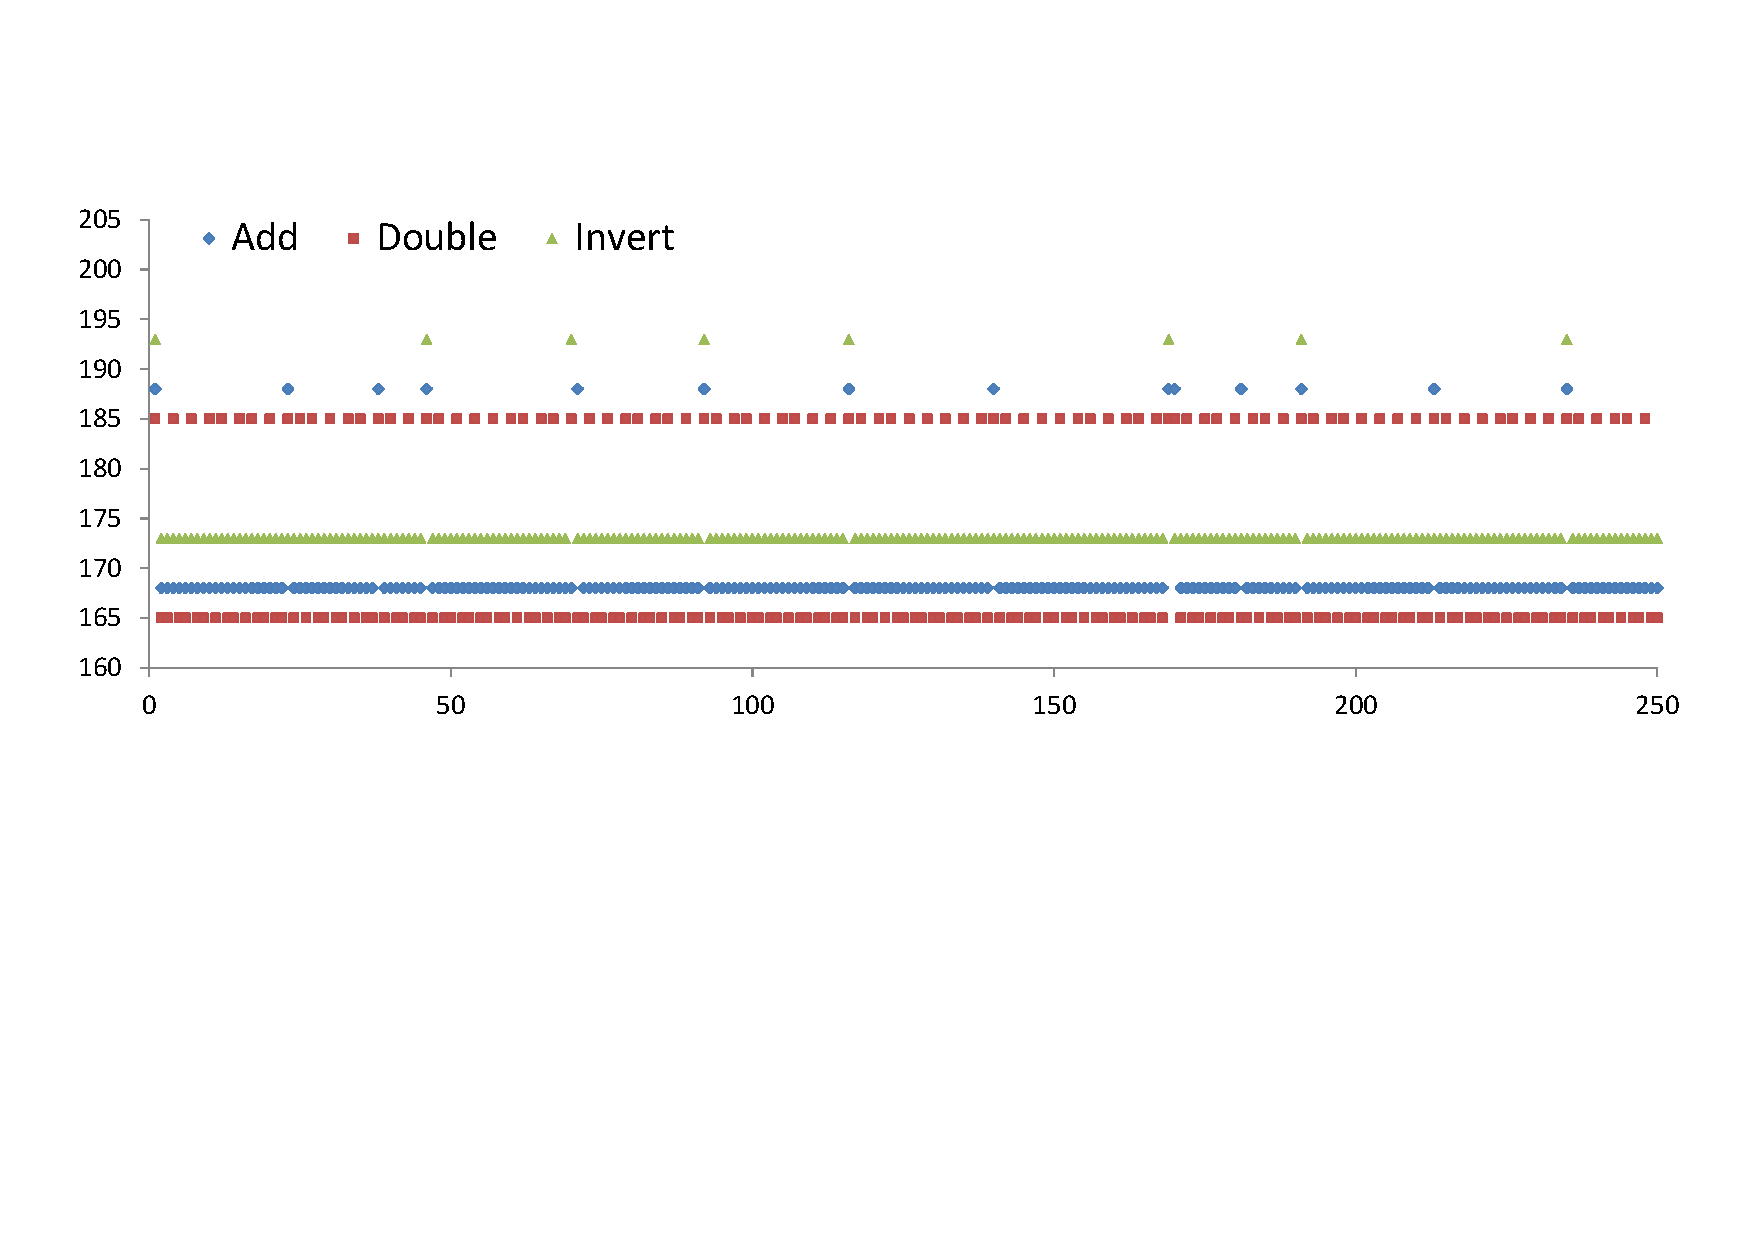
\includegraphics[width=\textwidth]{pic/slot2500.pdf}
%\caption{A fragment of the output of the Flush+Flush attack.} \label{fig1}
%\end{figure}
%
%
%%�����ʾ�����н��ͣ�
%%ʲô���Ŵ����ĸ�����
%%sample������ֵxx ��ʾ�����ʱ����ڣ�������ִ���ˡ�
%%Ȼ��for example�� ����ʱ���1�� ʲô�������ˣ������ĸ�������ִ���ˣ���˶�Ӧ��0����1��
%%Ȼ��ʱ���x����1��
%%����˵ʱ���x2 ����1��ͬʱinvert�����ˣ�˵����λ���ź�֮ǰ�෴��
%%ʱ���x3��δ����invert������λ��֮ǰ��ͬ��
%%
%%ʱ���x4�������������������Ĵ���
%%
%%����ʵ��k��ȣ���ȷ����x\%
%%
%%��ff����һ�����ߣ��õ�������õ�double add invert �������лָ�
%%Ȼ��ָ��ɹ����Ƕ��٣�
%%
%%
%%���
%
%


%
%
%\subsection{Lattice Attack}
%\label{latticeattack}
%%ʹ�������IJ��ŵ����
%%���ǵĽ���ǣ�
%%�����
%%����Ϊʲô����û������ȫ������Ϣ��������������ʵ������
%We apply our lattice attack to the curve secp256k1 in our experiments, and we assume that the Flush+Flush attack is perfect, which means we can correctly obtain the ``double-add-invert'' chain and recover all the information about the digits of the ephemeral key it contains.
%
%The HNP problem can be solved by exploiting both the CVP and SVP instances.
%However, the CVP problem does not have a polynomial time solution while the SVP problem has.
%So, with the growth of the dimension of the lattice, the time cost of finding the closest vector grows very fast.
% Actually, the CVP problem can be converted to the SVP problem,
%  so it is often solved through embedding the CVP into an SVP problem and using the polynomial time solution in practice.
%Therefore,
% in our experiments, we only demonstrate the result of using the SVP problem to solve the HNP instance.
%
% We use the BKZ algorithm implemented in \verb+fplll+~\cite{fplll} to solve the SVP problem.
%When solving an SVP instance, there are two outcomes that either we obtain the private key or a wrong answer.
% So we denote the success probability as the amount of successfully recovering the private key divided by the total number of the lattice attacks.
%We want to find the optimal strategy for our attack in terms of the following parameters:
%\begin{itemize}
%%\item CVP or SVP
% \item  the minimal value of $l$ (length of the consecutive bits of $k$)
% \item  the block size of BKZ
% \item  the lattice dimension
% %\item  pruning strategy (optional)
% %\item  total signature number
%\end{itemize}
%
%Thus we perform a number of experiments with different values of the parameters.
% In each case, we run $200$ experiments and compute the success probability.
%Because in Section \ref{sec:attack} the HNP problem introduced requires $l/2 - \log_{2}{3} -1 \geq 1$ to contain more than one bit information, the value of $l$ should be larger than $7$.
% But in our experiments, when $l = 8$, the private key can not be successfully recovered.
%  The reason is that the HNP instance contains not enough information in this case.
%So the minimal length of the consecutive bits of $k$ is set ranging from $9$ to $11$ in the experiments.
%When $l \geq 9$ or $l \geq 10$, the block size in BKZ is set $10$  and $20$.
%While $l \geq 11$, the block is set only $10$.
%The number of sequences of the consecutive bits for constructing the lattice denoted as $d$ is ranged from $50$ to $230$,
%i.e. the dimension of the lattice for the SVP is $d + 2$.
%
%\begin{table}[t]
%  \centering
%  \caption{The success probability of solving SVP with different parameters.}
%  \label{svp9}
%    \begin{tabular}{|c|m{0.5in}<{\centering}|m{0.5in}<{\centering}|m{0.5in}<{\centering}|m{0.5in}<{\centering}|m{0.5in}<{\centering}|}
%    \hline
%    \multirow{3}{*}{Dimension}&
%    \multicolumn{5}{c|}{Block size}   \\ %
%    \cline{2-6}
%    ~& \multicolumn{2}{c|}{$l \geq 9$} & \multicolumn{2}{c|}{$l \geq 10$} & $l \geq 11$  \\
%    \cline{2-6}
%    ~& 10 & 20 & 10 & 20  & 10 \\
%    %\hline
%  \hline
%  50 & 0  & 0  & 0 & 0 & 0   \\
%  \hline
%  60 & 0  & 0 & 0 & 0 &  3.0    \\
%  \hline
%  70 & 0  & 0  & 0.5 & 1.0  &  29.5    \\
%  \hline
%  80 & 1.0  & 1.5 & 4.0 & 8.5 &  49.0  \\
%  \hline
%  90 & 0.5  & 1.0 & 14.5 & 22.5 & 67.0   \\
%  \hline
%  100 & 0.5  & 4.0 & 21.0 & 33.5 & 70.5  \\
%  \hline
%  110 & 1.5  & 3.0 & 16.0 & 36.5 &  79.5 \\
%  \hline
%  120 & 2.0  & 4.5 & 21.5 & 35.0 &  77.5  \\
%  \hline
%  130 & 0.5  & 2.5 & 24.0 & 45.5 &  83.0  \\
%  \hline
%  140 &  3.0 & 8.0 & 29.0 & 46.0 &  88.5   \\
%  \hline
%  150 & 3.0  & 6.0 & 32.0 & 49.0 &  88.0  \\
%  \hline
%  160 & 2.5  & 13.0 & 27.5 & 49.0 &  94.0  \\
%  \hline
%  170 & 5.0  & 12.5 & 39.0 & 56.5 &  93.0  \\
%  \hline
%  180 & 3.5  & 11.5 & 37.0 & 57.0 &  97.0  \\
%  \hline
%  190 & 7.0  & 19.5 & 39.0 & 63.5 &  98.0  \\
%  \hline
%  200 & 9.5  & 26.0 & 46.0 & 66.0 &  99.0  \\
%  \hline
%  210 & 10.5  & 22.0 & 51.5 & 66.0 & 99.5   \\
%  \hline
%  220 & 15.0  & 29.0 & 51.0 & 72.5 & 100.0    \\
%  \hline
%  230 & 19.0  & 30.0 & 58.5 & 73.5 & 99.0  \\
%  \hline
%    \end{tabular}
%\end{table}
%
%Table \ref{svp9} shows the success probability for different dimensions and block sizes of solving the SVP instance in the
%             cases that the minimal length of the consecutive bits ranges from $9$ to $11$.
%As shown in the table, we successfully recover the private key of a 256-bit ECDSA only need $60$ sequences of consecutive bits with a success probability of $3.0\%$.
%These $60$ sequences come from up to $60$ signatures.
%Therefore we just need at most $60$ signatures to successfully recover the ECDSA private key.
%
%  For the fixed  minimal length of consecutive bits,
% increasing the dimension generally increases the probability of success.
%In some sense, as the dimension increases,
%     more information is being added to the lattice, and this makes the desired solution vector stand out more.
%Also, the higher block sizes perform with a higher success probability,
% as the stronger reduction allows them to isolate the solution vector better.
%  We believe that the success probability would be surely higher with the block size $30$ or the BKZ 2.0~\cite{bkz2}.
%
%When $l$ is fixed, to get a suitable success probability, attackers can either increase the dimension or use stronger algorithms (increasing the block size).
%However, increasing the dimension requires more signatures
% and enlarging the block size increases the computation time.
%So attackers can balance the two factors according to their resources and needs.
%
%The success probability also increases as the minimal length of consecutive bits increases.
%It is because more information is added to the lattice making it easier to search for the desired solution vector.
%But the increase of the minimal length would lead to requiring more signatures to obtain enough eligible sequences of consecutive bits.
% Because with the increase of minimal length, the probability of obtaining  a longer sequence of consecutive bits becomes lower.
%
%
%%\begin{table}[b]
%%  \centering
%%\begin{tabular}{|c|c|c|c|}
%%  \hline
%%  % after \\: \hline or \cline{col1-col2} \cline{col3-col4} ...
%%  dimension & 10 & 20 & 30 \\
%%  50 & 0 & 0 & 0 \\
%%  60 & 0 & 0 & 1.0 \\
%%  70 & 0.8 & 1.2  & 1.3 \\
%%  80 & 4.3 & 8.6 &  9.7 \\
%%  90 & 14.4 & 22.8 &  \\
%%  100 & 21.0 & 33.6 &  \\
%%  110 & 16.3 & 36.7 &  \\
%%  120 & 21.7 & 35.0 &  \\
%%  130 & 24.0 & 45.7 &  \\
%%  140 & 29.0 & 46.3 &  \\
%%  150 & 32.3 & 49.3 &  \\
%%  160 & 27.7 & 49.3 &  \\
%%  170 & 39.0 & 56.7 &  \\
%%  180 & 37.3 & 57.0 &  \\
%%  190 & 39.3 & 63.5 &  \\
%%  200 & 46.0 & 66.0 &  \\
%%  210 & 51.7 & 66.0 &  \\
%%  220 & 51.3 & 72.5 &  \\
%%  230 & 58.7 & 73.5 &  \\
%%  \hline
%%\end{tabular}
%%  \caption{the SVP result}\label{svp9}
%%\end{table}
%
%%Table \ref{svp8, svp9, svp10} show the probability of success when solving the CVP instance.
%%As shown from the table,
%%  the number of fragments of consecutive bits that we need to retrieve the private key of a 256-bit ECDSA is only $60$, less than the result of the SVP instance with the low block size.
%% The probability of success also increases as the the dimension or the block size increase.
%%Moreover, while the minimal length of consecutive bits increases, the probability of success becomes higher.
%%%�ټ�һ�λ򼸾�CVP�����SVP������бȽϡ�
%
%
%%The results of the SVP and CVP experiments (Appendix A) show that for fixed  minimal length of consecutive bits,
%% increasing the dimension generally increases the probability of success.
%%In some sense, as the dimension increases more information is being added to the lattice and this makes the desired solution vector stand out more.
%%The higher block sizes perform better,
%% as the stronger reduction allows them to isolate the solution vector better.
%%While the minimal length of consecutive bits increases, the the probability of success become higher.
%%Also we see that extensive pre-processing of the basis with more complex lattice reduction techniques provides no real benefit.
%\subsection{Comparison with Other Lattice Attacks}
%\label{compare}
%
% Generally,  to attack the ECDSA implementation with the wNAF representation,
%   the attackers target the scalar multiplication
%      and use cache side channel attacks to achieve the information about the ephemeral key $k$.
%Through side channels, attackers extract a ``double-add'' chain for the scalar multiplication.
%However,
% it is hard to directly recover the whole ephemeral key only from the ``double-add'' chain.
%%From the obtained information it can recover partial bits of the ephemeral key.
%Then, the private key recovery from incomplete information of $k$ is transformed into a problem that can be solved by lattice reduction,
%     such as an HNP or EHNP problem.
%Finally, the attackers recover the private key by solving the HNP or EHNP problem through being converted to the CVP/SVP problem in the lattice.
%
%
%
%\begin{table}[!t]
%  \centering
%   \caption{Comparison with previous attack methods}\label{compare1}
%\begin{tabular}{|c|m{90pt}|c|c|c|}
%  \hline
%  % after \\: \hline or \cline{col1-col2} \cline{col3-col4} ...
%  Methods & Exploited information & HNP or EHNP & \# of bits & \# of signatures \\
%  \hline
%  Benger et al. \cite{Benger2014} & LSB & HNP & 2 & 200 \\
%  \hline
%  Van de Pol et al. \cite{Van2015} & half positions of non-zero digits & HNP & 47.6 & 13 \\
%  \hline
%  Fan et al. \cite{Fan2016} & all positions of non-zero digits & EHNP & 105.8 & 4 \\
%  \hline
%  Wang et al. \cite{Wang2017} & positions of two non-zero digits and the length of the wNAF representation of $k$ & HNP & $\geq$ 2.99 & 85 \\
%  \hline
%  Ours & all positions and signs of non-zero digits & HNP & 153.2  & $\leq$ 60 \\
%%  \hline
%%  190 & 39.3 & 63.5 & & \\
%  \hline
%\end{tabular}
%\end{table}
%
%We compare the previous attack methods with ours in several aspects, and the result is shown in Table \ref{compare1}.
%Benger et al. \cite{Benger2014} got the least significant bits (LSBs) of the ephemeral key through the Flush+Reload attack
%although this is not all the information obtained from the side channel.
%Then they used the LSBs of many signatures to construct an HNP problem and
%successfully recovered the private key by solving the CVP/SVP instance of a specific lattice converted from the HNP problem.
%The number of bits extracted from each signature is very small, only an average of 2 bits information can be obtained,
%thus making it require more than $200$ signatures to recover a 256-bit private key with the probability being $3.5\%$.
%%In our work, we exploit information from the cache side channel to extract the consecutive bits at the position of every non-zero bits for the ephemeral key.
%%All the consecutive bits can be used to construct the lattice attack.
%%Therefore, we can get much more bits per signature and the number of signatures is decreased to recover the private key.
%% ��Ϊ��������200��ʵ��̫��û�б�Ҫ�Ƚ��ˡ�
%
%Van de Pol et al. \cite{Van2015} improved Benger's attack  relying on the property of some specific elliptic curves, that is the order $q$ of the base point is a pseudo-Mersenne prime which can be expressed as $2^n - \epsilon$, where $|\epsilon| < 2^p $, $p \approx n/2$ and $n$ is the length of $q$.
%With this property, this attack uses the information from the consecutive non-zero digits whose positions are between $p+1$ and $n$ extracted from the Flush+Reload attack, not only the LSBs.
%It is able to extract $47.6$ bits per signature on average for the secp256k1 curve and recover the private key with 13 signatures.
%Then they constructed an HNP instance using this information and
%successfully recovered the private key.
%Although this work greatly reduced the number of signatures needed to recover the private key,
%the information from the cache side channel is not fully utilized.
%But our work can use all the information from the cache side channel.
%Moreover, their work is only effective to some special curves,
% but ours can be applied to all the curves without any restriction.
%%This means that they can use about half of the information they got from the side channel.
%
%
%Fan et al.\cite{Fan2016} extracted all positions of digits from the Flush+Reload attack and took advantage of them to construct an EHNP instance.
%They managed to obtain on average 105.8 bits per signature for the secp256k1 curve
% and only need 4 signatures to recover the private key with the probability being $8\%$.
% Compared with their work, ours obtains more information about the ephemeral key, i.e. the sign of all non-zero digits, from the side channel by analysing the OpenSSL implementation.
%We can extract 153.2 bits information per signature.
%Although it uses more signatures to recover the private key in our lattice attack,
%theoretically, the number of signatures needed is less than Fan's if a more suitable lattice is constructed.
%
%Wang et al. \cite{Wang2017} obtained the positions of two non-zero digits and the length of the wNAF representation of $k$ from the Flush+Reload attack.
%They could obtain no less than 2.99 bits information per signature and exploit the HNP to recover the private key for the 256-bit curve using $85$ signatures.
%Obviously, our method obtains more information and uses fewer signatures to recover the private key.
%
%In summary, our method exploits both the signs and the positions  of the non-zero digits of the ephemeral key $k$ achieved from the Flush+Flush attack.
%It extracts the largest amount of information, on average $153.2$ bits per signature.
%In theory, the number of signatures needed to recover the private key is only $2$.
%However, due to the limit of our method of lattice construction,
% we need at most $60$ signatures, which is more than Fan's and Van de Pol's.
%One of our future work is to find an efficient lattice construction to solve the problem (e.g., an EHNP-based solution).
%
%%2017�꣬���Ŷӻ���science China information sciences �Ϸ���һƪ��ʹ��HNP�����£�
%%����һ��b����ڿ���(�����ۺ�����)
%%���DZ�����ڿ�������Ч��Ҫ�õġ�





























\section{Discussion}
\label{sec:discussion}

%\subsection{Scalar Multiplication in Other Cryptographic Libraries}
%Besides the OpenSSL library, there are many cryptographic libraries that implement the scalar multiplication.
%But not all of them use the wNAF representation.
%We introduce some implementations of the scalar multiplication in some popular cryptographic libraries.
%
%The mbed TLS \cite{polarssl} is an open source SSL library licensed by ARM Limited.
%It does not use the wNAF algorithm to represent the scalar.
%It uses a comb method that generates a sequence of bit-strings to represent the scalar $k$ so that every bit-string represents an odd number based on modifying the method in \cite{Hedabou2004ACM}.
%When computing the scalar multiplication, it traverses the sequence and directly indexes the value in the precomputed points to perform the addition.
%It does not use the invert function,
%and this representation is hard to attack by the cache side channels because all the elements of the sequence are not zero.
%
%Libgcrypt \cite{libgcrypt} is a cryptography library developed as a separated module of GnuPG.
%It directly uses the binary representation of the scalar instead of the wNAF representation to compute the scalar multiplication in the prime field.
%%Although it does not exploit the wNAF algorithm, it is vulnerable to the cache side channel attacks.
%To resist the side channel attacks, it performs an extra addition operation when the binary bit of the scalar is zero so that in every bit the double and addition are both performed.
%Therefore, lattice attacks to this library are invalid.

%Crypto++ Library \cite{cryptopp} is a free C++ class library of cryptographic algorithms and schemes.

%\subsection{The Method of Constructing Lattice Attacks}
%In our work, we construct an HNP instance using partial information about the $k$ obtained from the cache side channel attack.
% From the Inequation~\ref{lattice2}, the length of the most significant bits of $\lfloor\alpha t_i\rfloor$ is $l/2-\log_{2}{3} -1$.
%When constructing the lattice, it should contain the information about the most significant bits of $\lfloor\alpha t_i\rfloor$.
%Thus it requests $l/2-\log_{2}{3} -1 \geq 1$, so $l$ representing the minimal length of the consecutive bits needs to be larger than $7$.
%In practice, only when $l > 8$, we successfully recover the ECDSA private key in our experiments.
%However, the average length of the consecutive bits is $3$, which is much smaller than needed.
%This makes it impossible to use all the bits obtained through the cache side channel attack  to construct the lattice attack.
%Although in theory we only need $2$ signatures to recover the 256-bit private key,
% in practice we need at least $60$ signatures to get enough information satisfied the restriction on $l$ to construct the lattice attack.
%Therefore due to the restriction on $l$, we can not make full use of the information obtained from the cache side channel although we obtained $153.2$ bits information per signature on average.
%
%However, based on the work in~\cite{Nguyen2002} and \cite{Liu2013},
% in theory when the length of the consecutive bits is $2$, this sequence of  the consecutive bits can be used to construct the lattice attack.
%In our work, all the sequences of consecutive bits (except the least) obtained from the cache side channel satisfy $l \geq 2$,
% and the length the consecutive least significant bits is larger than $1$.
% That means at least $152.2$ bits information we obtained is valid and exploitable, only $1$ bit information may be discarded.
%Therefore, if we find an efficient way to construct the lattice attack, making full use of all the information of the consecutive bits,
%   the number of signatures required to recover the private key can be greatly reduced, even the best case only $2$ signatures is enough for a 256-bit private key.
%In theory, this result is better than the prior work in \cite{Fan2016} which theoretically needs 3 signatures for a 256-bit private key.
%This is what we are going to do next, finding a suitable and powerful method to construct the lattice attack.

%���ǵĹ����У�����ʹ����XX����
%���ǵķ�����ʲô���ƣ�l��Ҫ�ܴ�
%���ʲô������޷��������е���Ч���ݣ���Ҫʹ�úܶ��ǩ��
%���Ծ������ǻ�ȡ�����������ݣ��������ܹ�������á�

%�������Ͻ������ǻ�ȡ������������l>=3��������
%���ݲο����ף�ֻҪl=2�Ϳ��Ա��������и񹥻�
%��ˣ����ǻ�ȡ��������ȫ��������Ч���ݣ����Ա����õģ�����������Ҫ����������
%ֻ��Ҫ�ҵ����ʵķ���������񹥻����Ϳ��Գ���������ݣ��Ӷ���󽵵�����Ҫ��ǩ��������
%�����ϣ�����ֻ��Ҫ����ǩ������������fan��
%��Ҳ�����ǽ�����Ҫȥ���Ĺ������ҵ�һ�����ʵĹ����ķ�����

\subsection{The Imperfect Data from the Cache Side Channel}
\label{subsec:unperfect}
%֮ǰ�ĸ񹥻��������ǻ��������IJ��ŵ����ݽ��еġ�
%��ʵ���У����ŵ����ݲ����������ġ�
%���ڲ������IJ��ŵ���van�����˷���������Flush+reload��õ����ݣ��õ��Ľ����ǣ�
%��ˣ�ʹ�����ǵĸ񹥻���ʹ��fr����������ݣ�һ����Ҫ������ǩ����
%
%��������ʵ��ʱѡ����ʹ��ff����������fr�������ƣ����Ҳ������ͬ���ķ�����������з�����

Our lattice attack analysis is based on the perfect Double-Add-Invert chain, which means no errors exist in the chain.
But, achieving the perfect chain is almost impossible from the practical cache side channels.
Van de Pol et al.~\cite{Van2015} analysed the actual data obtained from the Flush+Reload attack.
Their statistical results show that $57.7\%$ of the obtained Double-Add chains are perfect.
We also can monitor the functions using the Flush+Reload attack,
 so the probability of the perfect Double-Add-Invert chain is also $57.7\%$, the same as Van de Pol's.
Thus, the actual number of signatures needed to recover the 256-bit ECDSA private key is $4$.

While in our experiments, we use the Flush+Flush attack to obtain the Double-Add-Invert chain.
Compared with Flush+Reload, the Flush+Flush is more easily to have errors, because the distributions of the execution time of the \verb+clflush+ instruction on cached and non-cached memory have some overlapping and the
difference in timing of this instruction is less.
So the probability to obtain the perfect chain is less than $57.7\%$.
We can re-measure the probability of obtaining the perfect chain using the same method with Van de Pol
 and achieve the actual number of needed signatures.


\subsection{The Precision of the Cache Side Channel Attacks}

Compared with Flush+Reload, the Flush+Flush can run in a higher frequency,
 because the execution time of the \verb+clflush+ instruction is less than the access time of the reloading operation and it can merge the two Flush stages into one to save the execution time.
So it obtains the Double-Add-Invert chain with less missing slots.
But the distributions of the execution time of the \verb+clflush+ instruction on cached and non-cached memory have
 some overlapping and the difference in timing of this instruction is less,
  so that it may make some wrong judgements on the Double-Add-Invert chain.
Therefore, for the obtained Double-Add-Invert chain,
 Flush+Flush and Flush+Reload produce different errors: Flush+Reload is more likely to produce the missing time slots, while Flush+Flush is more likely to produce the wrong observations.

We can choose the suitable time slot and monitoring addresses to reduce the wrong observations and
 using some optimisations to improve the Double-Add-Invert chain.
 In this way, the chain from Flush+Flush can be more accurate.
So in our paper, we use the Flush+Flush attack to show the availability of monitoring the invert function and obtain the Double-Add-Invert chain.

%For the Flush+Flush, we can eliminate the through careful configuration.










%\section{Related work}
\label{sec:relatedwork}
%我现在相关工作分成了两块,一块是部分密钥泄露攻击,一块是cache侧信道攻击,
%林老师您看下这块是否需要调整,增加哪些,删去哪些,或者结构调整?
%前面讲过的这里还需要再说吗?
\subsection{Partial Nonce Disclosure Attacks on DSA/ECDSA}
Several works have proposed different attacks that exploit partial nonce disclosure to recover long-term private keys of the signature algorithms.
Some of them focus on how to exploit the partial information efficiently to recover the private key.
 Some pay more attention to how to efficiently obtain the information about the ephemeral key.
Others want to  analyse the information obtained through some new methods and construct some appropriate lattice attacks to recover the private key.

% first
Boneh and Venkatesan \cite{boneh1996} initially investigated to use the partial information of the ephemeral key to construct an HNP problem and recovered the private key of Diffie-Hellman by solving it using the lattice reduction algorithm.
Howgrave-Graham and Smart \cite{HG2001} extended the work of Boneh and Venkatesan \cite{boneh1996} and  showed how to retrieve the DSA private key by  constructing an HNP instance from leaked LSBs and MSBs of the ephemeral key.
Nguyen and Shparlinski \cite{Nguyen2002} improved their method  and gave a provable polynomial-time attack that
      knowing the $l \geq 3$ LSBs , the $l+1$ MSBs  or any $2l$ consecutive bits of a certain number of ephemeral keys was enough for recovering the DSA private key.
 They recovered  a $160$-bit DSA key only using the $3$ LSBs of a certain number of ephemeral keys.
 Further they extended these results to ECDSA~\cite{Nguyen2003}.
Liu and Nguyen \cite{Liu2013} improved the results that only 2 LSBs were required for breaking a 160-bit DSA key.
In 2014, Benger et al. \cite{Benger2014} extended the technique in \cite{Nguyen2002} to use a different length of leaked LSBs for each signature.
 They recovered the secret key of OpenSSL's ECDSA implementation for the curve secp256k1 using about $200$ signatures.
Van de Pol et al. \cite{Van2015} exploited the property of the modulus in some elliptic curves so that they could use all of the information leaked in the top half of the ephemeral keys to construct the HNP instance, allowing them to recover the secret key after observing only $14$ signatures.
Fan et al. \cite{Fan2016} transformed the problem of recovering the secret key to the extended hidden number problem (EHNP)
  which was solved by the lattice reduction algorithm.
   Then the number of signatures needed was reduced to $4$.
   
%second
Brumley and Hakala \cite{Brumley2009} used an L1 data cache-timing attack to recover the LSBs of ECDSA ephemeral keys in OpenSSL 0.9.8k.
 They recovered a 160-bit ECDSA private key using the attack in \cite{HG2001} with collecting $2,600$ signatures ($8K$ with noise).
Analogously, Ac{\i}i{\c{c}}mez et al. \cite{Brumley2010} used an L1 instruction cache-timing attack to recover the LSBs of DSA ephemeral keys in OpenSSL 0.9.8l.
 It required $2,400$ signatures ($17K$ with noise) to recover a 160-bit DSA private key.
 Besides, both attacks required HyperThreading architectures.
In 2011, Brumley and Tuveri \cite{Brumley2011} mounted a remote timing attack on the implementation of ECDSA with binary curves in OpenSSL 0.9.8o.
 They obtained the MSBs of the ephemeral keys through the timing attack and recovered the private key after collecting information over 8,000 TLS handshakes.
Benger et al. \cite{Benger2014} and Van de Pol et al. \cite{Van2015} used the Flush+Reload technique to acquire the information of the ephemeral key.
Allan et al. \cite{Allan2016} improved the  results in \cite{Van2015} by using a performance-degradation attack to amplify the side-channel. The amplification allowed them to recover a 256-bit private key in OpenSSL 1.0.2a after observing only 6 signatures.
Genkin et al. \cite{Genkin2016} performed electromagnetic and power analysis attacks on mobile phones.
 They showed how to construct HNP triples when the signature uses the low $s$-value.
Pereida et al. \cite{Pereida2016} showed that the DSA implementation in OpenSSL is vulnerable to cache-timing attacks due to a programming error,
 and exploited the vulnerability to attack against SSH (via OpenSSH) and TLS (via stunnel).

%third
In 2013, Mulder et al. \cite{Mulder2013} took advantage of a template attack to recover some LSBs of the ephemeral key.
They improved the Bleichenbacher’s FFT-based (Fast Fourier Transform) attack by using BKZ for range reduction to solve the HNP problem.
Their attack could extract the entire private key using a 5-bit leak of the ephemeral key from 4 000 signatures.



%\cite{Zhang2017}
%Faug{\`e}re et al. \cite{jean2012}
%\cite{Gomez2019}
%\cite{}
%\cite{}
%\cite{}

\subsection{Cache Side Channel Attacks}
In 2002, Page \cite{Page2002} first described a theoretical chosen plaintext attack based on the collection of cache profiles.
One year later Tsunoo et al. \cite{Tsunoo2003Cryptanalysis} proposed the first practical implementation of cache attacks on the DES cryptographic algorithm.
The first practical cache side-channel attack on AES appeared in 2005 by Bernstein \cite{Bernstein2005Cache} showing that the table look up operations from different cache lines have different access times in an AES encryption.
Bonneau and Mironov’s study \cite{Bonneau2006} shows how to exploit cache collisions in AES as a source for time leakage.
In a similar attack, Osvik et al. \cite{Osvik2006} presented two spy processes that are able to monitor the cache usage: Evict+Prime and Prime+Probe.
Although the latter one proved to be significantly more efficient, both spy processes recovered the AES encryption key used by an OpenSSL server.
A few months later, Bonneau and Mironov \cite{joseph2006} and Ac{\i}i{\c{c}}mez and Ko¸c \cite{ac2006} presented new attacks targeting AES that exploited internal table look up collisions in the cache during the last and first rounds respectively.
Also,
in another study done by Gullasch et al. \cite{cachegame2011} flush+reload is used to attack AES encryption by blocking the execution of AES after each memory access.

Ac{\i}i{\c{c}}mez in \cite{Onur2007Yet} was the first one discovering that the instruction cache as well as the data cache leaked information when performing RSA encryption.
Brumley and Boneh performed a practical attack against RSA in \cite{Brumley2005Remote}.
Later Chen et al. developed the trace driven instruction cache attacks on RSA.
 Finally Yarom et al. were the first ones proposing a flush+reload attack on RSA using the instruction cache \cite{flushreload}.
  Then, again Yarom et al. used the Flush+Reload technique to recover the secret key from a ECDSA signature algorithm \cite{yarom2014recovering}.

Cloud computing systems became the next challenge for side-channel attack researchers.
In 2009, after Ristenpart et al. \cite{get-off-my-cloud} demonstrated that they were able to co-locate an attacker’s virtual machine (VM) with a potential victim’s VM with a success probability of 40\% in the Amazon EC2 cloud.
 Even further, the authors managed to recover keystrokes from the co-resident victim’s VM, showing that the cache side-channel attacks are both practical and applicable to real world scenarios.
The possibility of co-location fueled further research on new cache side-channel techniques and cache leakages in VMs.
For instance, Flush+Reload is used to attack AES \cite{Irazoqui2014} and RSA\cite{flushreload}.
At the same time, previous side-channel techniques such as Prime+Probe were also
adapted to work in virtualized settings by Zhang et al. \cite{YinqianZhang2012-cross-vm} and Liu \cite{liu2015last}.
They utilized a spy process to detect co-resident tenants and to recover ElGamal encryption keys.
Irazoqui et al. \cite{fine2014} recovered AES keys in virtualized environments with Bernstein’s attack.
Benger et al. \cite{Benger2014} demonstrated the viability of the Flush+Reload technique to recover ECDSA encryption keys,
and Van de Pol et al. \cite{Van2015} improved this work by using less signatures.
Fan et al. \cite{Fan2016} proposed a new way of extracting and utilizing information from the Flush+Reload attack.
Flush+Flush \cite{gruss2016flush} and Prime+Abort \cite{disselkoen2017prime+abort} are the variants of Flush+Reload.
They exploit different methods to observe the cache access patterns to recover the private key.


Brumley and Hakala \cite{Brumley2009} used an L1 data cache-timing attack to recover the LSBs of ECDSA nonces from the \verb+dgst+ command line tool in OpenSSL 0.9.8k.
 They collect $2,600$ signatures ($8K$ with noise) and use the Howgrave-Graham and Smart \cite{HG2001} attack to recover a 160-bit ECDSA private key.
In a similar vein, Ac{\i}i{\c{c}}mez et al. \cite{Brumley2010} use an L1 instruction cache-timing attack to recover the LSBs of DSA nonces from the same tool in OpenSSL 0.9.8l, requiring $2,400$ signatures ($17K$ with noise) to recover a 160-bit DSA private key.
 Both attacks require HyperThreading architectures.


%Several works have been presented to attack the ECDSA implementation with the wNAF representation.
% Generally, the attackers target the implementation of scalar multiplication
%  and use cache side channel attacks to achieve the information about the ephemeral key $k$.
%Through the cache side channels attackers can get a "double-and-add" chain for the scalar multiplication.
%However, because the wNAF representation of $k$ is a sequence of signed digits,
% it is hard to directly recover the whole ephemeral key just depending on the "double-and-add" chain.
%From the obtained information it can only determine the position of the non-digital bits and some least significants bits of the ephemeral key.
%Hence attackers exploit the incomplete information of $k$ to transform the problem of private key recovery into one that can be solved by lattice, such as HNP or EHNP problem.
% Then the attackers retrieve the private key by solving the HNP or EHNP problem through being converted to the CVP/SVP problem in the lattice.
%
%%攻击一般有以下几个步骤,对标量乘法进行攻击,首先是通过cache侧信道攻击获取有关k的一些信息,
%%然后通过侧信道获取的信息,得到k的某些bit位的信息,或者k的信息。
%%通过获得到的信息,将求解私钥的问题转化为可以通过格来求解的问题,进而通过求解格困难问题来获取私钥。
%%ECDSA wNAF 部分密钥泄露攻击
%
%%找到一个共同的点,论文在这个点,或这几个点相关,然后进行分析。
%%
%%首先对这些论文按某些特点进行分类
%%在每个类别里,每个工作和本文进行详细对比,
%%它是怎么实现的,用了什么技术,达到了什么效果
%%本文的情况如何
%%从数据获取,到数据分析方法,然后结果进行比较
%%相同点,不同点
%
%Benger et al. \cite{Benger2014} presented an attack to the ECDSA implementation with the wNAF representation in 2014.
%They got the least significant bits (LSBs) of the ephemeral key through the Flush + Reload attack
%although this is not all the information obtained from the side channel.
%Then they used the LSBs of many signatures to construct a HNP problem and
%successfully retrieved the private key by solving the CVP/SVP instance of a specific lattice converted from the HNP problem.
%The number of bits extracted from each signature is very small, only an average of 2 bits information can be obtained.
%Thus made it require more than 200 signatures to recover a 256-bit private key
%with the probability being 3.5\%.
%In our work, not only do we get more information from the cache side channel,
% but also we can exploit it to extract the consecutive bits at the position of every non-zero bits for the ephemeral key.
%All the consecutive bits can be used to construct the lattice attack.
%Therefore, we can get much more bits per signature and the number of signatures is decreased for retrieve the private key.
%
%In 2015, van de Pol et al. improved Benger's attack.
%Their method relied on the property of some specific elliptic curves, that is the order $q$ of the base point is a pseudo-Mersenne prime.
%This prime can be expressed as $2^n - \epsilon$, where $|\epsilon| < 2^p $, $p \approx n/2$.
%With this property, this attack can use the information from the consecutive non-zero digits whose positions are between $p+1$ and $n$ extracted from the Flush + Reload attack, not only the LSBs.
%This means that they can use about half of the information they got from the side channel.
%Then they constructed a new HNP instance using this information and
%successfully retrieved the private key.
%According to this paper, it is able to extract 47.6 bits per signature on average for the secp256k1 curve and recover the private key with 13 signatures.
%Although this work greatly reduced the number of signatures needed to recover the private key,
%the information from the cache side channel is not fully utilized.
%But our work can use all the information from the cache side channel.
%Moreover, their work is only effective to some special curves,
% but ours can be applied to all the curves without any restriction.
%%the curves with the special property is just a small part of all the curves. This method of constructing the HNP instance can not be extended to other kinds of curves.
%
%Both of the two works exploited the HNP instance to retrieve the ECDSA private key.
%While Fan et al.\cite{Fan2016} proposed a new method to
% extract information from the Flush + Reload attack.
%It takes advantage of all positions of digits to construct an EHNP instance.
%The EHNP problem is solved in the same way as the HNP problem,
%being converted into the SVP problem on the lattice.
%They managed to obtain on average 105.8 bits per signature for the secp256k1 curve
% and only need 4 signatures to retrieve the private key with the probability being 8\%.
% Compared with their work, ours obtains more information about the ephemeral key, i.e. the sign of all non-zero digits, from the side channel by analysing the OpenSSL implementation.
%Furthermore, we transform the information of the wNAF representation to the binary information of $k$ to construct the lattice attack for the first time.
%We can extract xx bits information per signature.
%Although it uses more signatures to retrieve the private key through our lattice attack,
%theoretically the number of signatures needed is less than Fan's if a suitable lattice is constructed.
%
%2017年,范团队还在science China information sciences 上发了一篇,使用HNP的文章,
%这是一个b类的期刊。(交叉综合新兴)
%需要在这里和它进行对比吗,还是这三篇就够了。
%我们比这个期刊的文章效果要好的。
%
%
%%In 2017, \cite{Wang2017} give a lattice attack on the ECDSA implementation in the
%%latest version of OpenSSL which uses the wNAF method to implement the scalar multiplication, using
%%only a small fraction of information of the double-and-add chain of the ephemeral key.
%%we only need to know the positions of the second non-zero digit and the last non-zero
%%digit (from the higher index) together with the length of the chain rather than obtaining a perfect one
%%from the side-channel attack.
%%
%%
%%In 2015, \cite{Cao2015} presents two Lattice-Based Differential Fault Attacks Against ECDSA with wNAF Algorithm.
%%
%%In 2016, \cite{Dahmun2016}  extend the famous Howgrave-Graham and Smart lattice attack when the nonces are blinded by the addition of a random multiple of the elliptic-curve group order or by a random Euclidean splitting.
%
%%In 2015, van de Pol et al. improved Benger's attack.
%%They also used the Flush + Reload method to attack the scalar multiplication.
%%They used the position information of the non-zero digits extracted from the side channel, not only the LSBs.
%%Their method relied on the property of some specific elliptic curves, that is the order $q$ of the base point is a pseudo-Mersenne prime.
%%This prime can be expressed as $2^n - \epsilon$, where $|\epsilon| < 2^p $, $p \approx n/2$.
%%With this property, this attack can use the information from the consecutive non-zero digits whose positions are between $p+1$ and $n$ extracted from the side channel.
%%This means that they can use about half of the information they got from the side channel.
%%Then they constructed a new HNP instant using this information and
%%successfully retrieved the private key.
%%According to this paper, it is able to extract 47.6 bits per signature on average for the secp256k1 curve and recover the private key with 13 signatures.
%%This work greatly reduced the number of signatures needed to recover the private.
%%Although it used half of the information more than the Benger's, the information from the cache side channel is not fully utilized.
%%Moreover, the curves with the special property is just a small part of all the curves. This method of constructing the HNP instance can not be extended to other kinds of curves.









\section{Conclusion}
\label{sec:conclusion}
In this paper, we demonstrate a practical attack on the ECDSA algorithm implemented by OpenSSL with the scalar multiplication using the wNAF representation.
We improve the original cache side channel attack by adding an extra monitor to the invert function and get the extra information about the sign of all non-zero digits of the ephemeral key.
Then we exploit a new method to get the consecutive bits of the ephemeral key at the position of the non-zero digits through the ``double-add-invert" chain obtained by the cache side channel attack.
From the side channel, we obtain $153.2$ bits of information per signature for the secp256k1 curve.
We construct a lattice attack using the HNP problem to recover the ECDSA private key.
This is the first work to obtain the information about the sign of the non-zero digits of the ephemeral key and make use of it to recover the ECDSA private key.
We implement our method to attack the secp256k1 curve.
The experiments show that we successfully recover the private key only using $60$ signatures.

\zf{please check the page limitation}




%%
%% The acknowledgments section is defined using the "acks" environment
%% (and NOT an unnumbered section). This ensures the proper
%% identification of the section in the article metadata, and the
%% consistent spelling of the heading.

%\begin{acks}
%To Robert, for the bagels and explaining CMYK and color spaces.
%\end{acks}


%
% ---- Bibliography ----
%
% BibTeX users should specify bibliography style 'splncs04'.
% References will then be sorted and formatted in the correct style.
%
% \bibliographystyle{splncs04}
% \bibliography{mybibliography}
%

%%
%% The next two lines define the bibliography style to be used, and
%% the bibliography file.
\bibliographystyle{ACM-Reference-Format}
\bibliography{bib/Reference}


\end{document}
\endinput
%%
%% End of file `sample-sigconf.tex'.
